% This must be in the first 5 lines to tell arXiv to use pdfLaTeX, which is strongly recommended.
\pdfoutput=1
% In particular, the hyperref package requires pdfLaTeX in order to break URLs across lines.

\documentclass[11pt]{article}

% Remove the "review" option to generate the final version.
\usepackage{acl2023-mod}
\usepackage{booktabs} % Add this line to include the booktabs package
% Standard package includes
\usepackage{times}
\usepackage{latexsym}
\usepackage{float} % For [H] option
\usepackage{placeins} 
\usepackage{natbib}


% For proper rendering and hyphenation of words containing Latin characters (including in bib files)
\usepackage[T1]{fontenc}
% For Vietnamese characters
% \usepackage[T5]{fontenc}
% See https://www.latex-project.org/help/documentation/encguide.pdf for other character sets
\usepackage{graphicx}
% This assumes your files are encoded as UTF8
\usepackage[utf8]{inputenc}

% This is not strictly necessary, and may be commented out.
% However, it will improve the layout of the manuscript,
% and will typically save some space.
\usepackage{microtype}

% This is also not strictly necessary, and may be commented out.
% However, it will improve the aesthetics of text in
% the typewriter font.
\usepackage{inconsolata}
\usepackage{enumitem} % for customizing lists

\usepackage{linguex}


% If the title and author information does not fit in the area allocated, uncomment the following
%
%\setlength\titlebox{<dim>}
%
% and set <dim> to something 5cm or larger.

\title{Analyzing Xenophobic and Anti-Immigrant Rhetoric in Matteo Salvini's Tweets: A Computational Approach}

% Author information can be set in various styles:
% For several authors from the same institution:
% \author{Author 1 \and ... \and Author n \\
%         Address line \\ ... \\ Address line}
% if the names do not fit well on one line use
%         Author 1 \\ {\bf Author 2} \\ ... \\ {\bf Author n} \\
% For authors from different institutions:
% \author{Author 1 \\ Address line \\  ... \\ Address line
%         \And  ... \And
%         Author n \\ Address line \\ ... \\ Address line}
% To start a seperate ``row'' of authors use \AND, as in
% \author{Author 1 \\ Address line \\  ... \\ Address line
%         \AND
%         Author 2 \\ Address line \\ ... \\ Address line \And
%         Author 3 \\ Address line \\ ... \\ Address line}

\author{Vittorio Ciccarelli $\vert$ 3118588\\
  \href{mailto://Vittorio.Ciccarelli@hhu.de}{Vittorio.Ciccarelli@hhu.de}}

\begin{document}
\maketitle

\begin{abstract}
Detecting hate speech on social media has become crucial over the last few years. Platforms like Twitter are often used by political figures in order to expand their political discourse to a wider audience. Their communication, however, might sometimes convey populist and xenophobic stances. The present research aims to analyze Italian politician Matteo Salvini's tweets to investigate, with the help of Natural Language Processing (NLP) techniques, how he discusses and frames immigrants and immigration as a phenomenon, and whether nuances of xenophobia can be found in his tweets. Results showed that immigration-related issues are among the most discussed topics in Salvini’s Twitter communication, and are generally framed negatively and as a concern to society. These results are in line with previous qualitative studies and highlight Salvini's use of populist and anti-immigration rhetoric.

\end{abstract}
\noindent \textbf{Keywords:} Matteo Salvini, hate speech, Twitter, political discourse, xenophobia, immigration, NLP.

\section{Introduction}

The number of people using Twitter\footnote{For the sake of simplicity and clarity, the social media platform formerly known as Twitter, now referred to as 'X', will be denoted as 'Twitter' throughout this paper.} as a source of news and information has grown at an exponential rate in recent years \citep{doi:10.1080/19331681.2023.2293868}, and as a result, an increasing number of political figures has started to exploit the platform to broadcast their political discourse to a wider audience \citep{YAQUB2017613}, gain public acclaim and propagate their political ideologies \citep{doi:10.1177/2056305119891220}. However, the promotion of specific political beliefs by politicians on these platforms can sometimes escalate and contribute to hate-speech, xenophobia and racism. 

Italian politician Matteo Salvini, for instance, has frequently been accused of xenophobia and anti-immigrant rhetoric, especially due to his frequent use of hashtags like \textit{\#chiudiamoiporti} (close the ports) and \textit{\#primagliitaliani} (italians first) \citep{evolvi2019emotional}. Detecting and preventing hate-speech, xenophobia and abusive language online has thus become increasingly important \citep{DBLP:journals/corr/ParkF17}. In this regard, Natural Language Processing (NLP) is gaining significant attention \citep{capozzi2020contro}, with various competitions like SemEval-2019 and SemEval-2020 striving to find automated solutions for hate-speech detection \citep{jahan2023systematic}.

The present research is intended as a quantitative analysis of Matteo Salvini's tweets. In particular, we will employ state-of-the-art language models, frequency distribution analysis and sentiment and emotion classification to provide a comprehensive computational analysis of Salvini's tweets on immigration-related topics, with the aim of uncovering traces of hate speech, xenophobia and anti-immigrant rhetoric.  
\section{Background}

\subsection{Hate Speech and Social Media}

Research on social medias has showed that such platforms, while offering great freedom of expression, can also facilitate the increase of cases of online racism, both in covert and overt forms \citep{sukanya2023racism}. Studies in this area also focus on the role that social media plays in reflecting as well as shaping public opinions about different groups and minorities, highlighting how crucial they are in the production and reproduction of stereotypes \citep{lorenzetti2020anti}.
Over the last few years, a great deal of  research has focused on the arduous task of hate speech detection on social media platforms, primarly by making use of the increasingly cutting-edge techniques of Natural Language Processing (NLP), such as employing machine learning (ML) and deep learning (DL) algorithms to identify racist content on Twitter, or by classifying tweets as being “racist” or “nonracist” \citep{sukanya2023racism, kwok2013locate}.

In the context of Italy, projects such as “Contro L’Odio” \citep{capozzi2020contro} focused on monitoring and contrasting hate speech against immigrants with the aid of computational linguistics techniques. \citet{sanguinetti2018italian} proposed a Twitter corpus of about 6,000 annotated tweets for the purpose of hate speech detection against immigrants.
Following the same line, HATE-ITA \citep{nozza2022hate} presented a set of multilingual models aiming to improve hate speech detection in italian text. 
This high level of interest in the topic of hate speech and racism detection, especially in the context of social media platforms, proves that it is indeed a hot topic in nowadays' society. 

\subsection{The Case of Matteo Salvini}
 
Italian Interior Minister Matteo Salvini is known for his explicitly anti-immigration and anti-Islamic positions. Lega, the political party under his leadership, has a history of regional secessionism and anti-southernism (formerly called Lega Nord). Since Salvini took the lead, it has switched its focus from secessionism to nationalism, directing its opposition rhetoric no longer against southerners, but against migrants and in particular the Islamic community, repeatedly using slogans such as 'stop immigration!' and 'defend the Italians from invasion' to frame immigrants as a threat to Italy's security \citep{cervi2020exclusionary}. 

There is extensive research on Salvini that highlights his xenophobic and Islamophobic positions. Cervi (\citeyear{cervi2020exclusionary})’s comparative analysis of Italy
and Spain, for instance, focused on Islamophobia and highlights how Salvini and his party monopolise the discourse on immigration and portray Muslims in a negative manner. On the same line, Amnesty International's (\citeyear{amnesty2018}) and (\citeyear{amnesty2019}) Hate Barometer reports that Matteo Salvini's main target during election campaigns tended to be Muslims (right after the more general category of immigrants), often referred to as the 'muslim threat'.

Further qualitative research such as that of \citet{cervi2020populists} analysed Matteo Salvini's speeches on the topic of immigration and highlighted how he uses a typically populist narrative, describing migrants as 'others' in order to legitimate repressive policies. Part of the research on Salvini also highlights the extent to which he makes large use of Twitter to spread his political, anti-immigration and Islamophobic messages. \citet{lorenzetti2020anti}, for instance, offers a comparative analysis of speeches and tweets from Donal Trump and Matteo Salvini, showing how they share strong anti-immigration positions and an extensive use of social media to spread their message and legitimise the use of racist and disciminatory language. \citet{reggi20237}, on the same line, carried out an appraisal and emotional analysis of a sample of Salvini’s tweets, according to which his populist discourse portrays migrants, and in particular the Muslim community, as the main out-group, while \citet{evolvi2019emotional} highlighted how Salvini uses provocative hashtags such as \textit{\#closeports} to generate emotional reactions in his supporters, and how he indiscriminately mixes Islam and migration on social media, presenting both as 'dangerous others' and threats to
Italian society.

This considerable amount of literature on Matteo Salvini illustrates how he makes use of his populist rhetoric, especially on Twitter, to promote anti-immigration and islamophobic stances.


\section{Research Questions}

For the purpose of this analysis, we focused on the following research questions:
\begin{enumerate}[label=\textbullet, align=left, leftmargin=*]
    \item How frequently does Matteo Salvini talk about immigration-related topics in his tweets?
    \item What are common n-grams (unigrams, bigrams, trigrams) used by Salvini in tweets about immigration, and do they contain xenophobic or racist language?
    \item What is the sentiment distribution in Salvini's tweets regarding immigration and immigrants?
    \item What emotions are most frequently expressed in Salvini's tweets about immigration-related topics?
    \item How do this research’s findings compare with previous studies on his rhetoric?
\end{enumerate}
To address such research questions, a multi-step NLP pipeline was implemented to analyse a dataset of Matteo Salvini's tweets.




\section{Data}

The dataset that was used for this research is an open source dataset retrievable on the github repository \href{https://github.com/galatolofederico/deep-salvini}{DeepSalvini}, an artificial intelligence-based generative language model trained on Matteo Salvini's corpus of tweets with the aim of reproducing tweets in the same manner as he would write them. The dataset consists of a text file containing exactly 46424 tweets, covering a time period from 2011 (the year Salvini first joined Twitter) to 2019. Within the file, each line corresponds to exactly one tweet and the tweets are separated from each other by a new line character. As we can see from this example, the original data included extensive metadata:

\begin{quote}
\ex. 50611293534695425 2011-03-23 18:34:07 +0200 <matteosalvinimi> \textit{Ecco il mio nuovo twitter} :-)
\end{quote}

Therefore, the very first step was to clean the data by removing unnecessary information such as tweet ID, timestamp, username etc. To achieve this, Regular expression \citep{aho1991algorithms}  was used to return all the content following <matteosalvinimi>. 
The cleaned version of the tweet we saw in (1), for instance, would thus be:

\begin{quote}
\ex. \textit{Ecco il mio nuovo twitter} :-)
\end{quote}

\section{Methodology}

Once the metadata was removed, we performed topic modeling, an unsupervised machine learning technique that extracts and identifies underlying topics from unstructured data \citep{blei2012probabilistic}, to identify the most salient topics discussed by Matteo Salvini on his Twitter and investigate whether topics related to the issue of immigration and migrants featured prominently among them. 
For this purpose, we decided to implement topic modeling using BERT (Bidirectional Encoder Representations from Transformers) \citep{devlin2018bert}, in particular the \href{https://huggingface.co/sentence-transformers/distilbert-multilingual-nli-stsb-quora-ranking}{distilbert-multilingual-nli-stsb-quora-ranking} model. To carry out topic modeling with BERT, four steps are necessary: (1) generate embedding representations of the tweets using the pre-trained sentence transformer, (2) employ the UMAP (Uniform Manifold Approximation and Projection) algorithm for dimensionality reduction purposes \citep{mcinnes2018umap}, (3) utilize the HDBSCAN (Hierarchical Density-Based Spatial Clustering of Applications with Noise) algorithm to cluster tweets that are similar into groups \citep{mcinnes2017hdbscan} and (4) extract topic representations through use of c-TF-IDF (class-based Term Frequency-Inverse Document Frequency) \citep{joachims1997probabilistic}.

Once these steps were performed, the obtained topics were interpreted and the ones considered to be related to immigration and immigrant groups were selected. The tweets belonging to these selected topics became the focus of the analysis.
Using the spaCy \citep{spacy2} library, the selected immigration-related tweets were tokenized and stop-words were removed in order to compute a frequency distribution to identify the most common n-grams (unigrams, bigrams and trigrams) and investigate whether nuances of racism or xenophobic language were to be found, as well as to understand Matteo Salvini's framing of immigration and immigrants in general\footnote{the same process of computing n-grams was also performed on the complete dataset for comparability}. As a final step, the feel\_it model \citep{bianchi2021feel} from Hugging Face was employed, allowing for Sentiment Classification and Emotion Classification on Italian text, and providing binary sentiment labels (positive and negative) and multi-class emotion classifications including ’joy’, ’anger’, ’sadness’, and ’fear’, to analyse the distribution of emotions and sentiment in the immigration-related tweets, enabling us to gain an insight into the emotional tone Salvini uses when discussing such topics. 


\section{Analysis of the results}

\subsection{Topic Modeling}

\begin{table}[ht]
\centering
\scalebox{0.62}{ % Adjust the scaling factor as needed
\begin{tabular}{@{}rrl@{}}
\toprule
Topic & Size & Representative Words \\
\midrule
-1 & 28366 & che\_la\_il\_non\_salvini \\
150 & 907 & tasse\_pagare\_le\_fiscale\_tax \\
138 & 861 & europa\_euro\_salvini\_europea\_ue \\
122 & 816 & immigrazione\_immigrati\_profughi\_clandestina\_sono \\
176 & 552 & galera\_carcere\_detenuti\_delinquenti\_penitenziaria \\
77 & 508 & roma\_piazza\_com\_pic\_twitter \\
69 & 484 & pic\_twitter\_olio\_latte\_com \\
184 & 470 & governo\_salvini\_non\_il\_che \\
79 & 435 & scuola\_insegnanti\_scuole\_azzolina\_studenti \\
141 & 423 & milano\_milan\_com\_facebook\_twitter \\
209 & 348 & live\_https\_videos\_salviniofficial\_facebook \\
160 & 326 & su\_diretta\_rete\_sarò\_compagnia \\
157 & 295 & rai\_su\_tre\_diretta\_uno \\
64 & 279 & isis\_islam\_islamico\_islamici\_terroristi \\
192 & 261 & amici\_buona\_buongiorno\_buon\_buonanotte \\
81 & 251 & sicilia\_palermo\_siciliani\_clandestini\_immigrati \\
194 & 240 & twitter\_pic\_com\_26maggiovotolega\_grazie \\
201 & 230 & votare\_referendum\_voto\_lega\_vota \\
74 & 229 & virus\_coronavirus\_il\_https\_emergenza \\
181 & 202 & senato\_dal\_intervento\_diretta\_mio \\
123 & 193 & libia\_ong\_nave\_immigrati\_libica \\
\bottomrule
\end{tabular}
}
\caption{20 most frequent topics (topic -1 contains the outliers)}
\label{tab:tab1}
\end{table}



\begin{figure*}[t]
  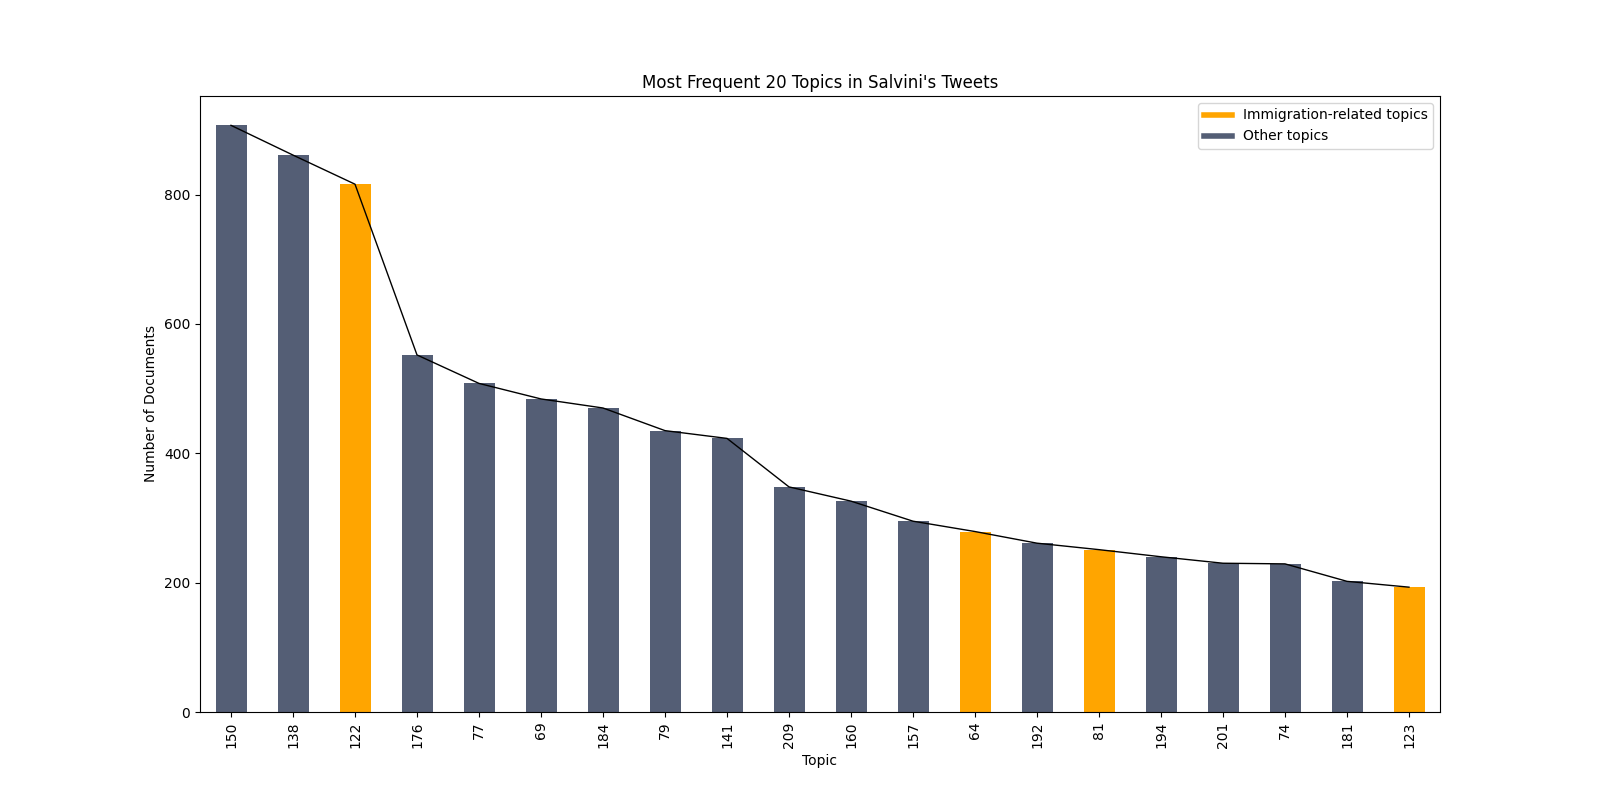
\includegraphics[width=1.0\linewidth]{topics.png}
  \caption{The 20 most frequent topics in Salvini’s corpus of tweets. The orange color indicates topics which were identified as being immigration-related }
  \label{all-scores}
\end{figure*}



Topic modeling on Salvini’s dataset revealed that out of the 20 most frequent topics, several are related to immigration and migrants. As we can see in Table \ref{tab:tab1}, the third most recurrent topic (topic 122)\footnote{Since Topic -1 consists of the outliers, we consider it at index 0} concerns immigration and immigrants in general. Topic 64 (the 13th most frequent) deals with Islam, terrorism and Muslims, while topics 81 (the 15th most frequent) and 123 (the 20th most frequent) are respectively about immigrants landing in Sicily and NGOs dealing with immigration (see Appendix \ref{figures} for word cloud representation of the topics). 
These results show Salvini's thematic emphasis on immigration and immigration-related issues. In addition, topics 64 and 123 reflect Amnesty International's (\citeyear{amnesty2018}) Hate Barometer’s results, according to which Muslims and Islam are Salvini’s main target after the general category of “immigrants”.
Out of the 46424 tweets that comprise the dataset, 28366 were classified as belonging to  Topic -1 (the outliers) while 1539 is the number of tweets we analysed as being related to immigration after grouping all the tweets belonging to topics 122, 64, 81, 123, which are the four immigration-related topics we identified in the twenty most frequent ones.

\subsection{Word Frequency Distribution}

\begin{figure*}[t]
  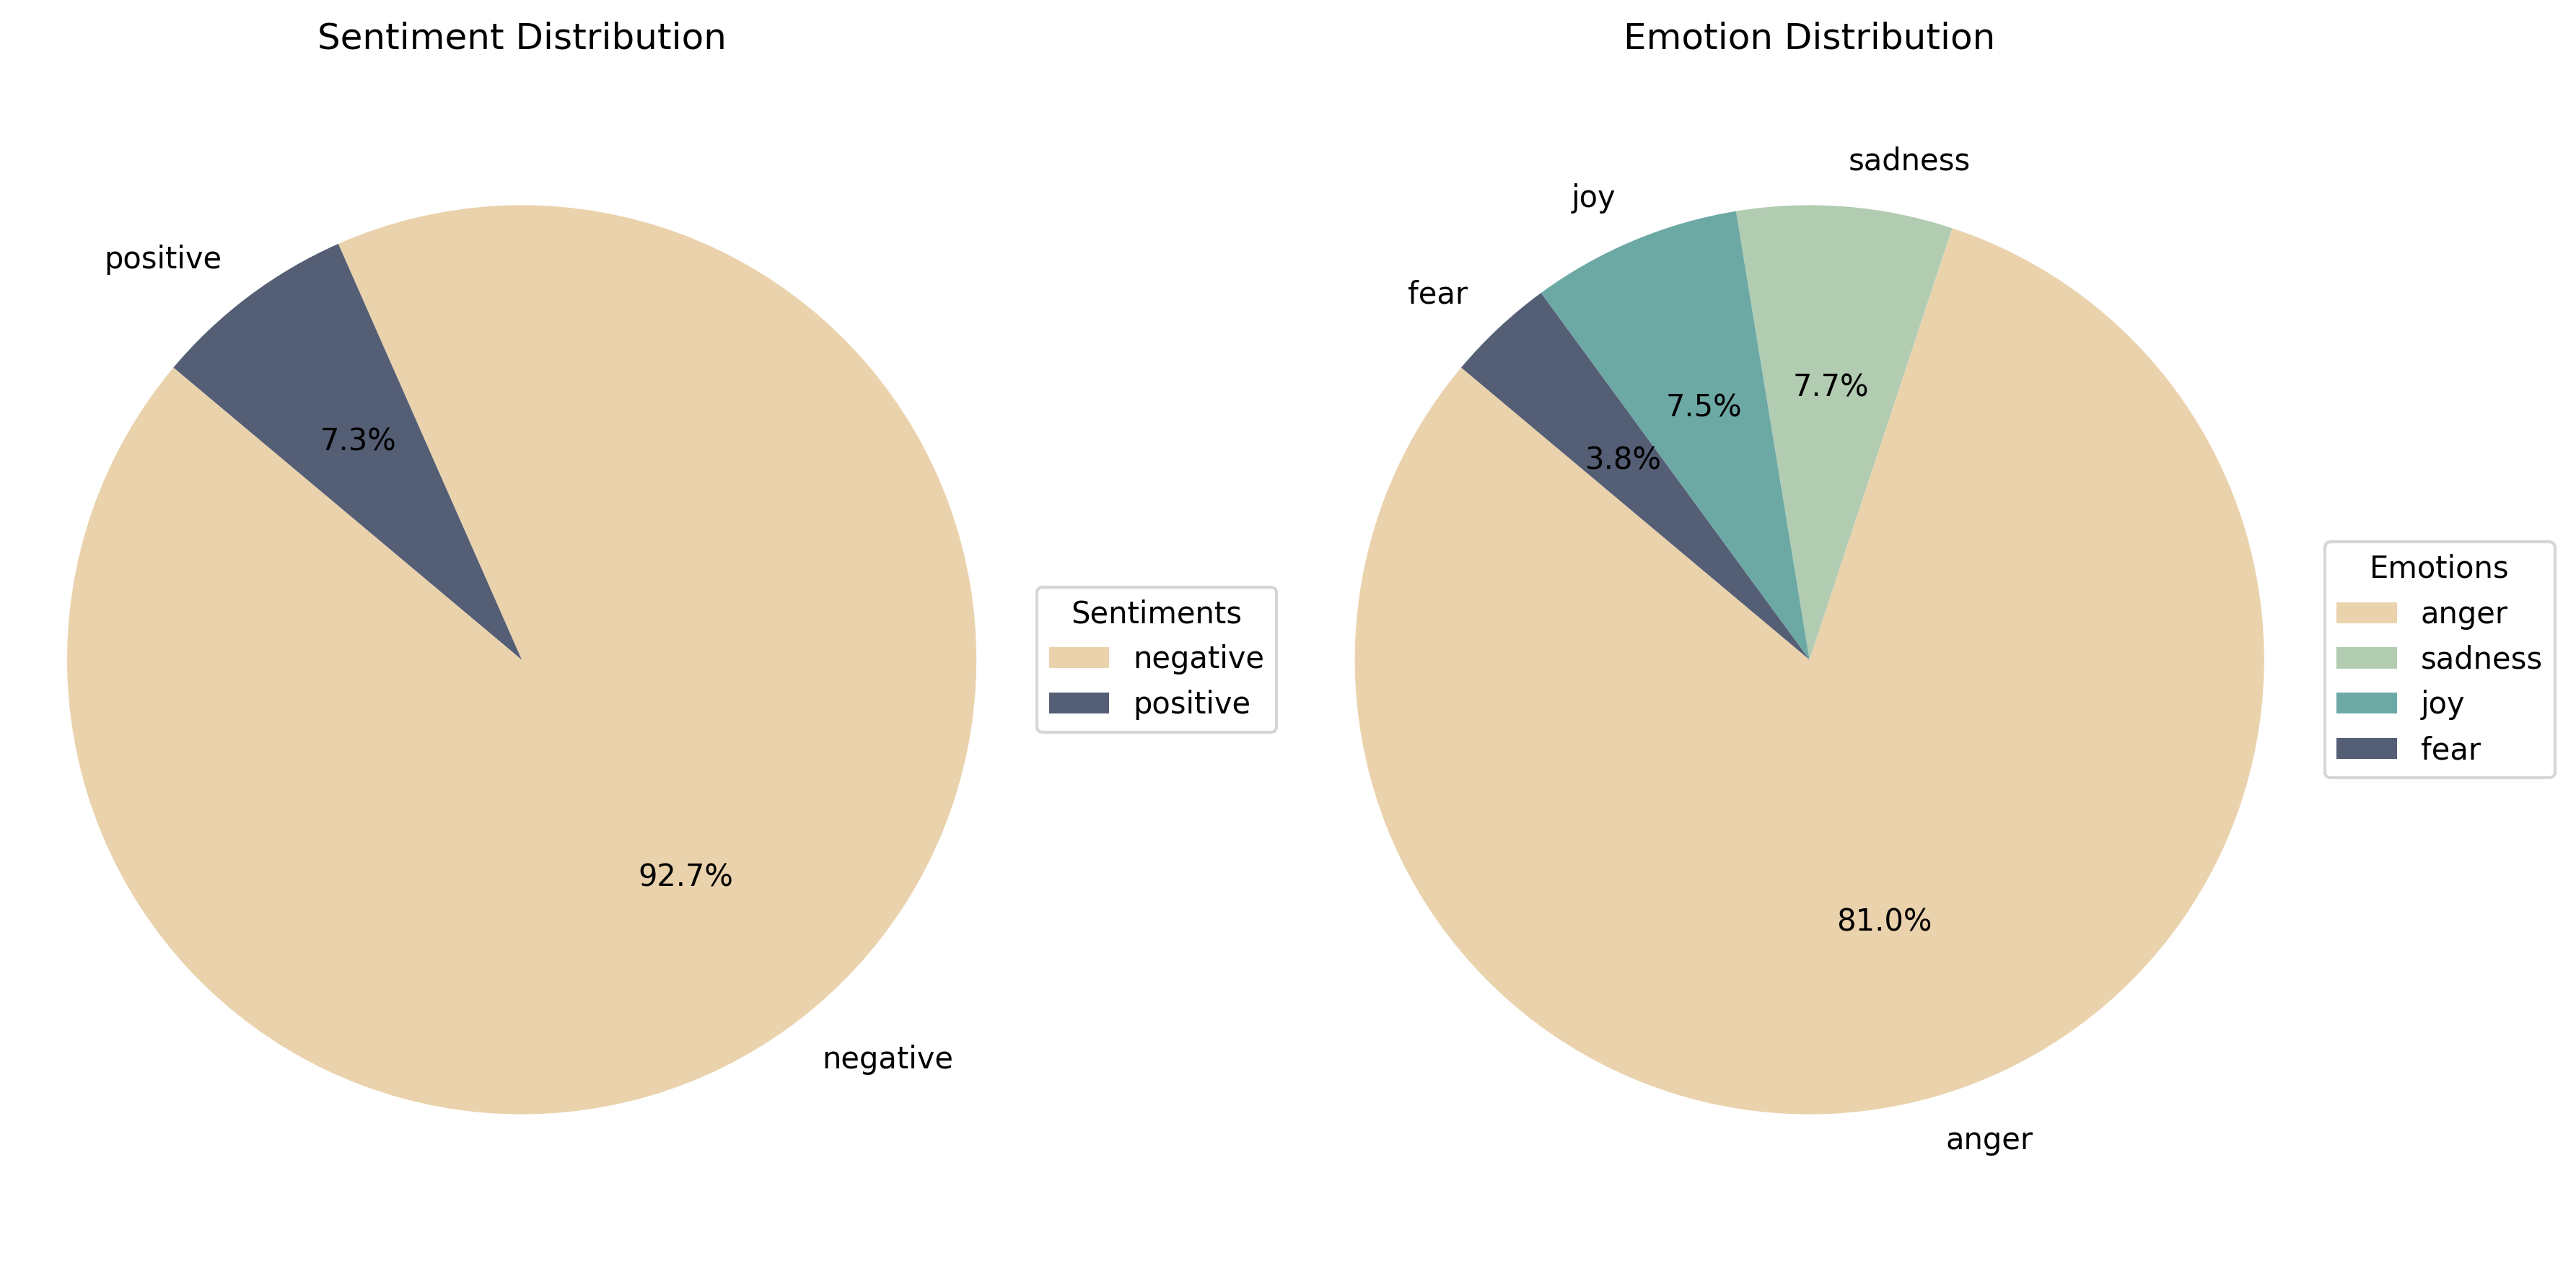
\includegraphics[width=1.0\linewidth]{sentiment_and_emotion_pie_charts_with_legends.png}
  \caption{Sentiment and Emotion distribution over the immigration-related tweets}
  \label{sentiment-emotion}
\end{figure*}

Among the most frequent unigrams over the whole dataset (see Appendix \ref{figures} for n-grams frequency distributions), "immigrati" (immigrants) figured as the 26th most frequent word, while "clandestini" (clandestines) figures as the 38th most frequent one. In the 50 most frequent bigrams, “immigrazione clandestina” (illegal immigration) figured at position 29. From a further exploration of the 100 most frequent unigrams and bigrams we could identify other constructions such as “prima italiani” (italians first) and the hashtag "\#primagliitaliani"(\#italiansfirst), reportedly used by Salvini to protest against immigrants \citep{evolvi2019emotional}. Although no relevant trigram was found among the 50 most frequent ones, a deeper analysis of the 100 most frequent trigrams allowed us to capture associations such as “business immigrazione clandestina” (illegal immigration business), “reato immigrazione clandestina” (illegal immigration crime) and “europa campo profughi” (europe refugee camp). These preliminary findings seem to confirm that immigration and migrants are among the most discussed entities in Salvini’s political discourse on Twitter.
The same frequency distribution analysis over the filtered set of immigration-related tweets highlighted that: “immigrati” (immigrants) and “immigrazione” (immigration) figure as the 2nd and 3rd most frequent tokens, followed by “italia” (italy) and “italiani” (italians),  evoking Salvini’s populist tendency to create a manichean opposition between the “us” (italians) and the “others” (immigrants) reported by \citet{cervi2020populists}. Other frequent unigrams are “clandestino” (clandestine), “rifugiato” (refugee), as well as “ONG” (NGO), “Islam”, “Muslims” and “problem”. 
Among the most frequent bigrams, “immigrazione clandestina” (illegal immigration) figures as the most frequent one. Other frequent bigrams are “immigrati irregolari” (illegal immigrants), “terrorismo islamico” (islamic terrorism), “reato immigrazione” (immigration crime), “fuori controllo” (out of control). Lastly, the two trigrams with the highest frequency distribution were again “business immigrazione clandestina" (illegal immigration business) and "reato immigrazione clandestina" (illegal immigration crime), together with "campo profughi europa" (europe refugee camp), "italia campo profughi" (italy refugee camp), "porti italiani chiusi" (italian ports closed). These findings appear to confirm the assumption that Salvini’s Twitter communication frames immigration as a crime and an out-of-control problem, immigrants as illegal entities and a threat to social stability, while portraying Italy as Europe’s refugee camp.

\subsection{Sentiment and Emotion Classification}



The last step of out analysis involved employing the \href{https://github.com/MilaNLProc/feel-it}{feel\_it} model for sentiment and emotion classification of italian text.
Sentiment classification highlighted a stark negative sentiment associated with the set of immigration-related tweets, with 92.7\% of them being classified as negative, while only 7.3\% was classified as positive. Emotion classification, on the same lines, reports anger as the dominant emotion, present in 81.02\% of the tweets, followed by sadness (7.67\%), joy (7.47\%) and fear (3.83\%). These results are indicative of a polarized rhetoric with strong negative sentiment and predominantly negative emotional responses surrounding immigration-related issues.


\section{Conclusion}

This quantitative study of Matteo Salvini's Twitter aimed at investigating the way in which the politician relates to immigrants and immigrant-related issues in his political discourse through the use of a comprehensive natural language processing (NLP) pipeline, with the ultimate aim of searching for nuances of hate speech and anti-immigration rhetoric, and to eventually obtain results that are in line with previous both quantitative and qualitative analyses on the same topic.
The results of the topic modeling process revealed the centrality of migrant and immigration issues in Salvini's political discourse on social media Twitter.
The frequency analysis of n-grams revealed that terms related to immigration and migrant groups appear among the most frequent terms over the entire dataset, and that some of them tend to connote immigrants and immigration in a negative and problematic way, framing them as a threat or problem to society, thus emphasising Salvini's anti-immigration stance.
Sentiment and emotion classification  showed that Salvini's emotional tone is predominantly negative, with anger being the most prevalent emotion associated with tweets about migrants and immigration. Overall, our findings appear to be consistent and in line with the results obtained from previous quantitative and qualitative analyses on Salvini's political discourse and his use of Twitter to propagate his political message, especially on the issue of immigration, which is framed as a threat and societal burden, reflecting his populist, xenophobic and anti-immigrant narrative.

\section{Limitations and Future Research}
Despite the promising results obtained with this research, we are aware of the limitations of our approach. The dataset, for instance, is limited to Salvini's tweets over a specific timeframe and may not be fully representative of his rhetoric. Methodologically, on the other hand, the topic modeling process could have placed other immigration and migrant-related tweets in distinct clusters that escaped our analysis, thus causing us to lose valuable content. Additionally, we are unaware of possible biases introduced by the topic modeling process or the emotion and sentiment classification model. Future research should explore alternative models for detecting xenophobia and hate speech. One promising approach would be employing annotators to label Salvini's dataset specifically for xenophobic and anti-immigration rhetoric. This annotated data could then be used to fine-tune existing pre-trained models for this specific task. Given the sensitivity and complexity of hate speech detection, continuous research and development of advanced techniques are crucial to finding effective solutions in this field.




% Entries for the entire Anthology, followed by custom entries
\bibliography{references}
\bibliographystyle{acl_natbib}



\appendix

\section{Data Access}

Project work and data are accessible under: \href{https://osf.io/dt39z/}{DOI 10.17605/OSF.IO/DT39Z} or this \href{https://github.com/wtto1206/HATE-SALVINI/tree/main}{github repository}. 

\section{Figures and Graphs} \label{figures}

\begin{figure}[H]
    \centering
    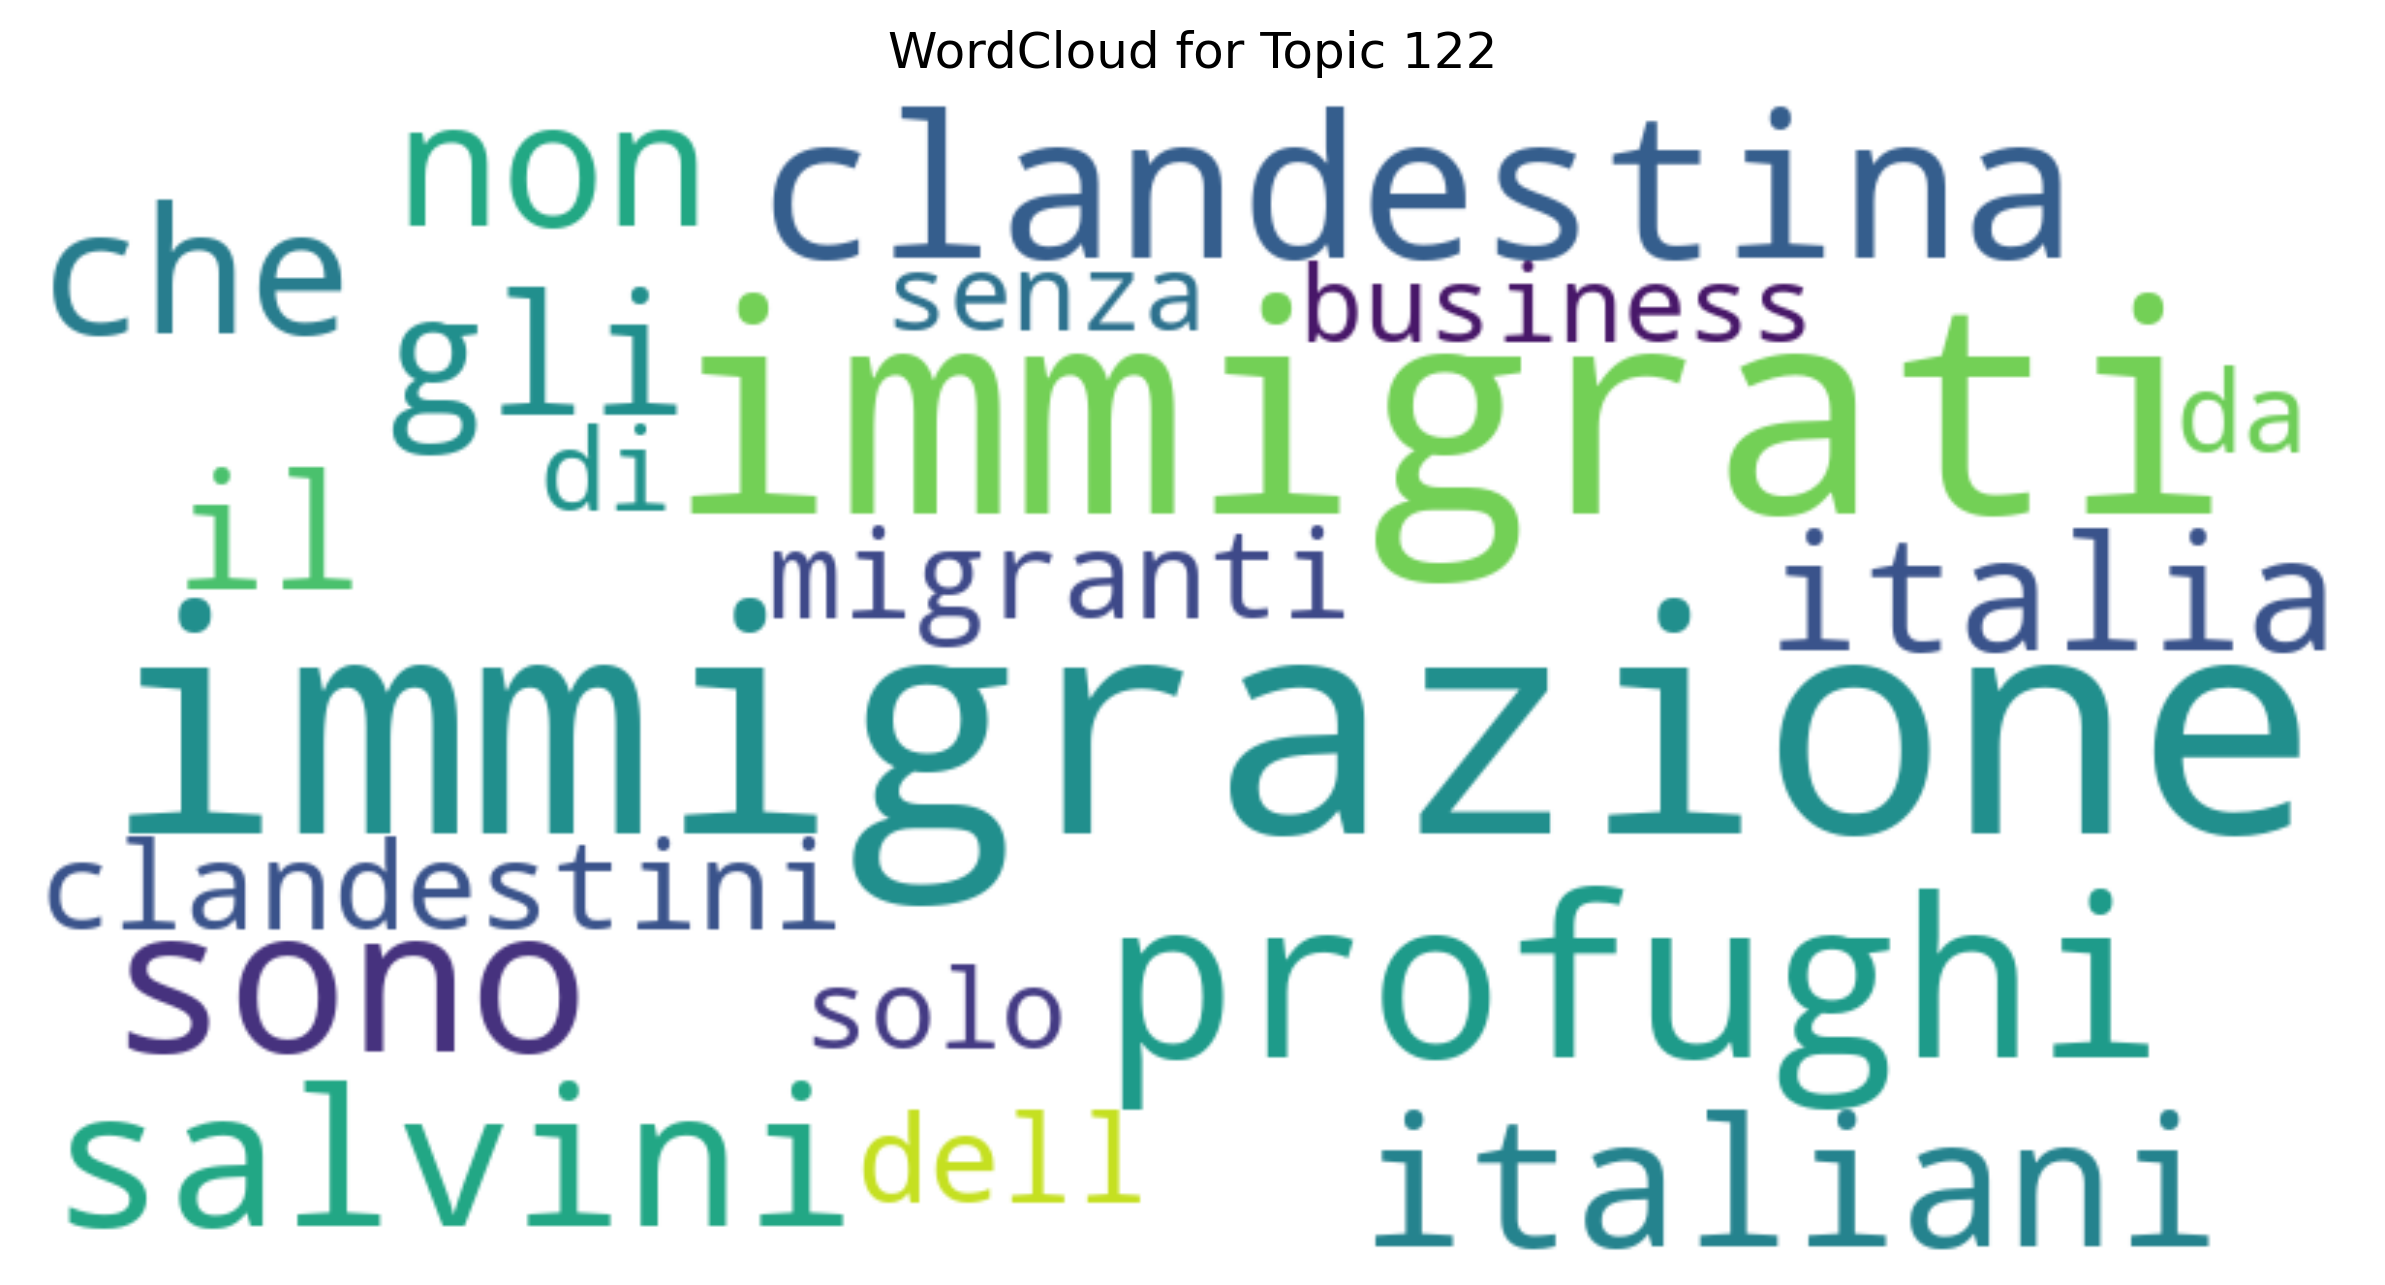
\includegraphics[width=1\linewidth]{wordcloud_topic_122.png}
    \caption{Word cloud representation of topic 122 (third most frequent topic}
    \label{fig:topic122}
\end{figure}

\begin{figure}[H]
    \centering
    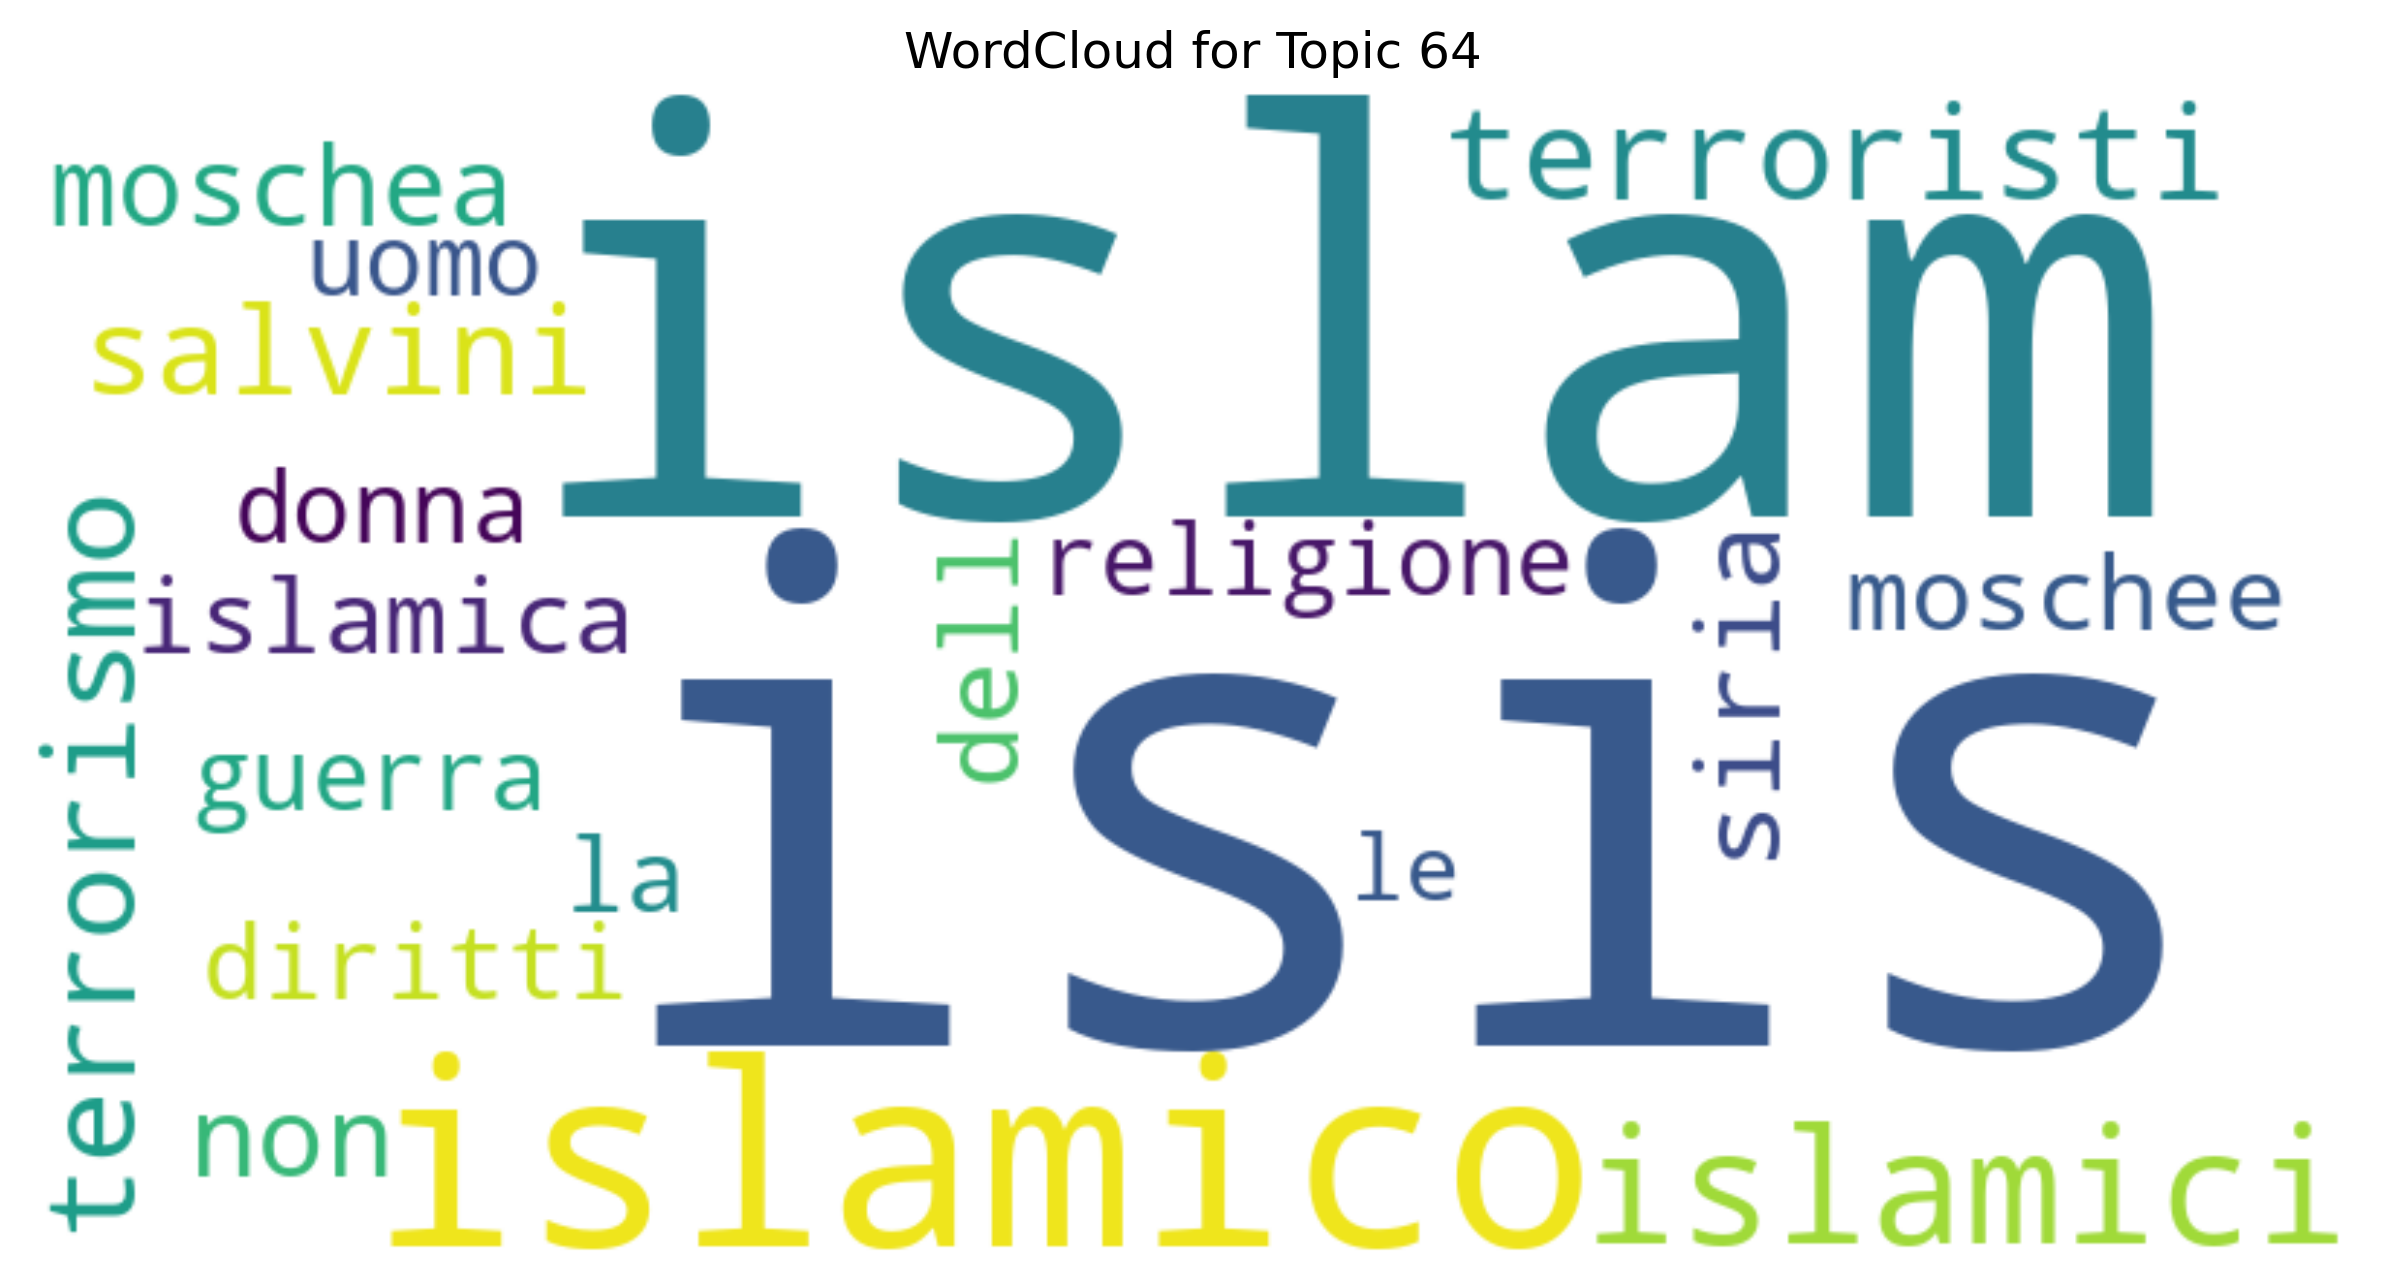
\includegraphics[width=1\linewidth]{wordcloud_topic_64.png}
    \caption{Word cloud representation of topic 64 (16th most frequent topic}
    \label{fig:topic64}
\end{figure}

\begin{figure}[H]
    \centering
    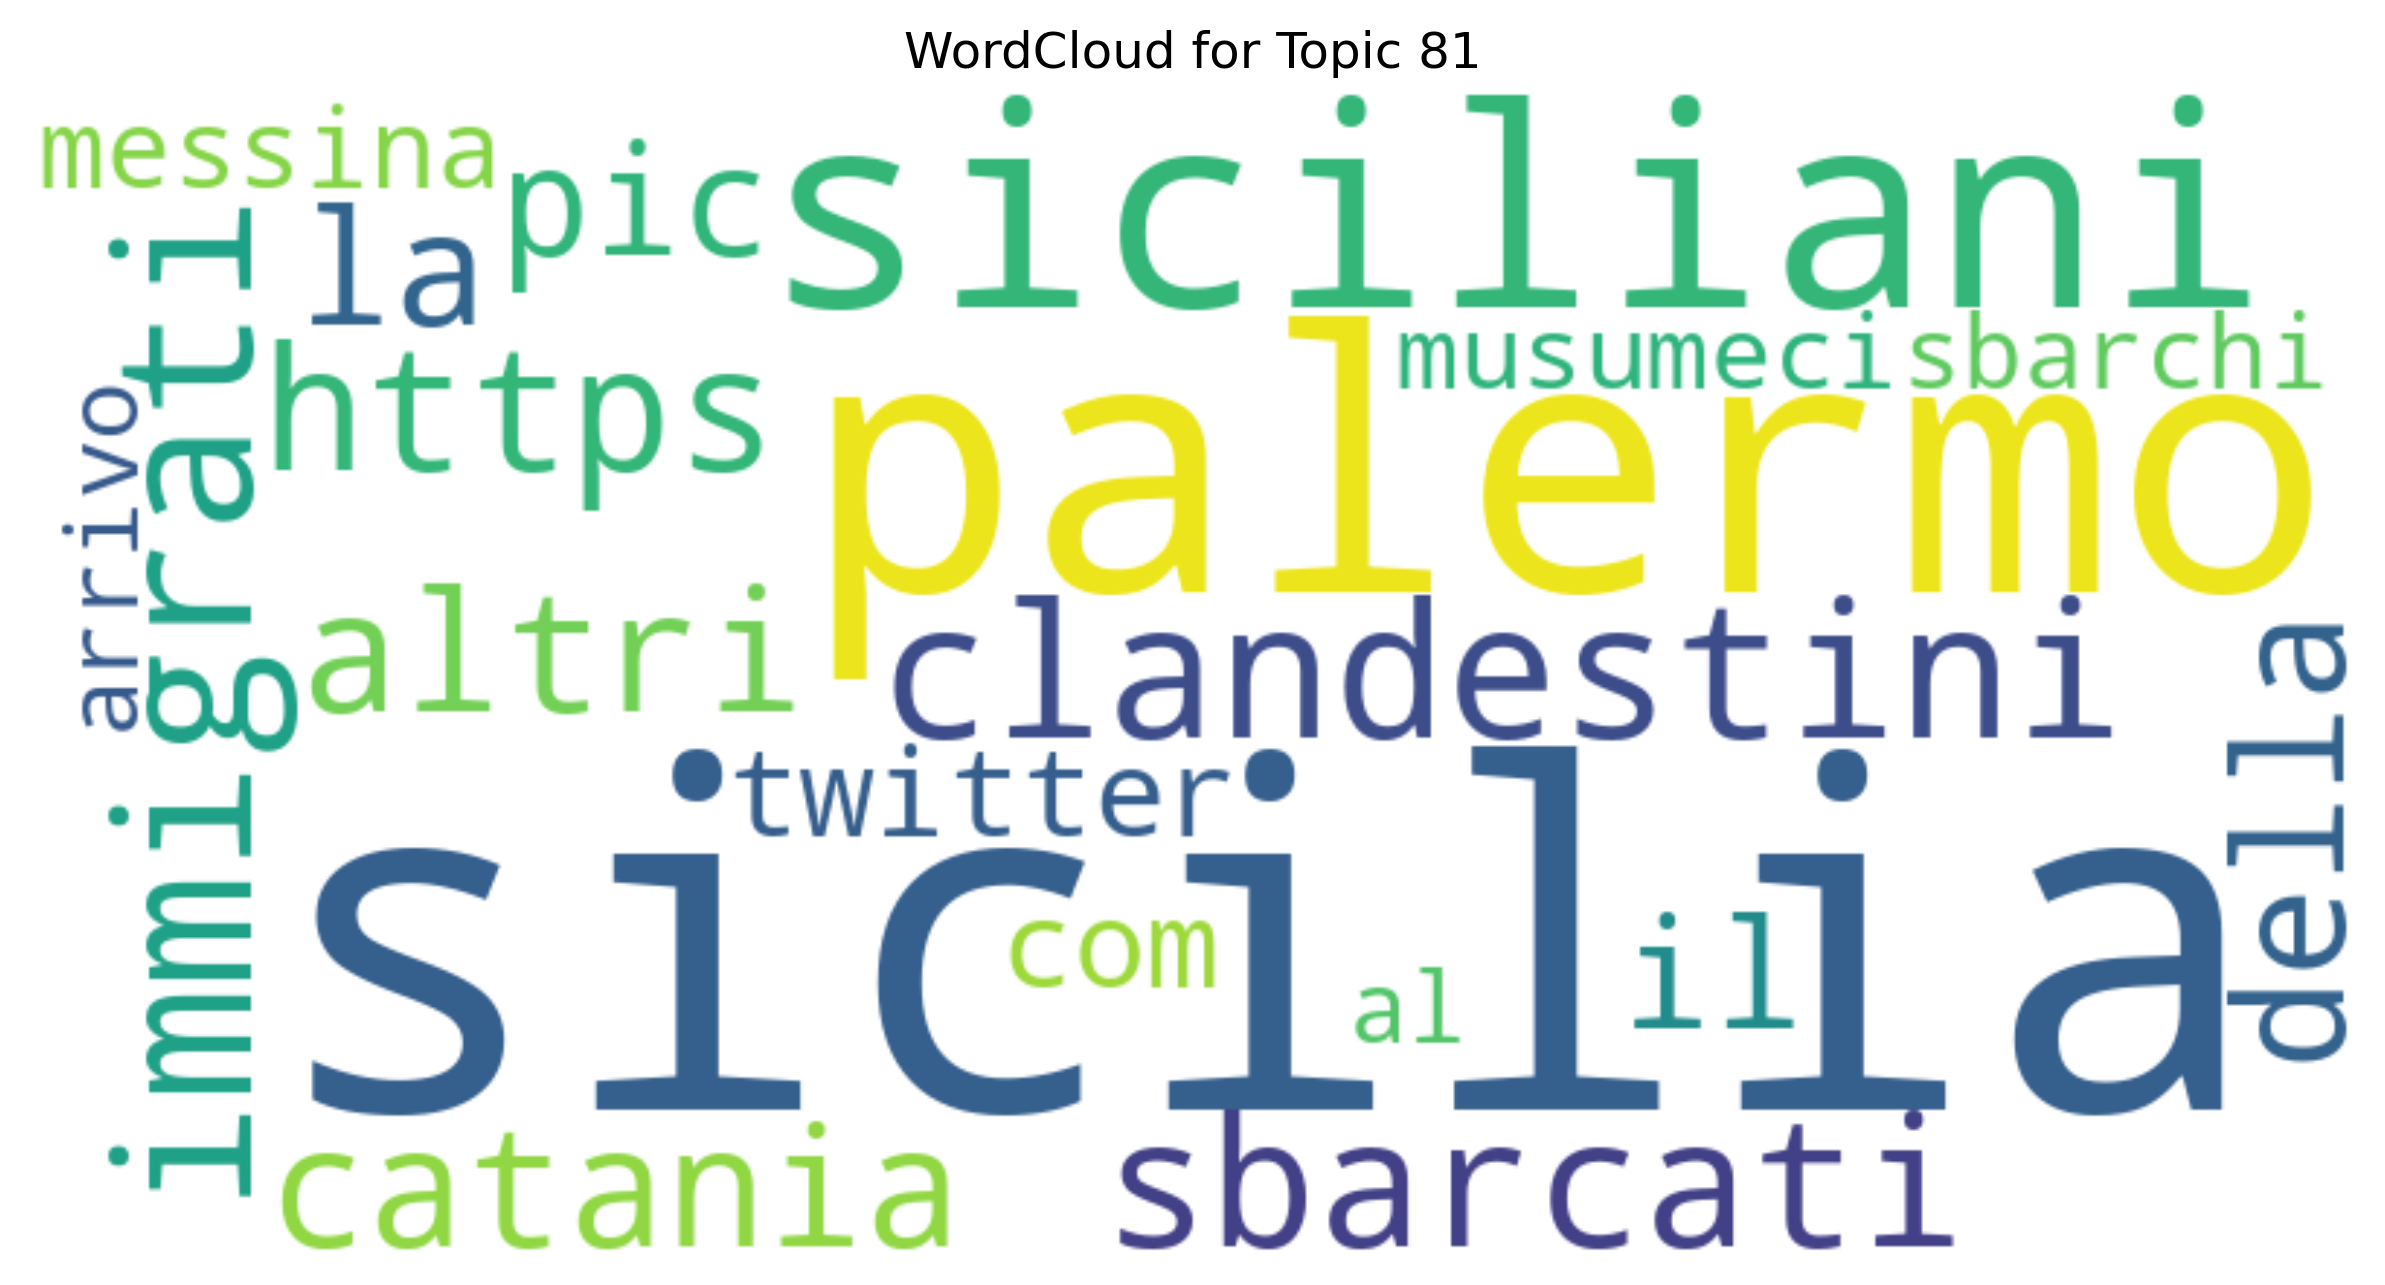
\includegraphics[width=1\linewidth]{wordcloud_topic_81.png}
    \caption{Word cloud representation of topic 81 (15th most frequent topic}
    \label{fig:topic81}
\end{figure}

\begin{figure}[H]
    \centering
    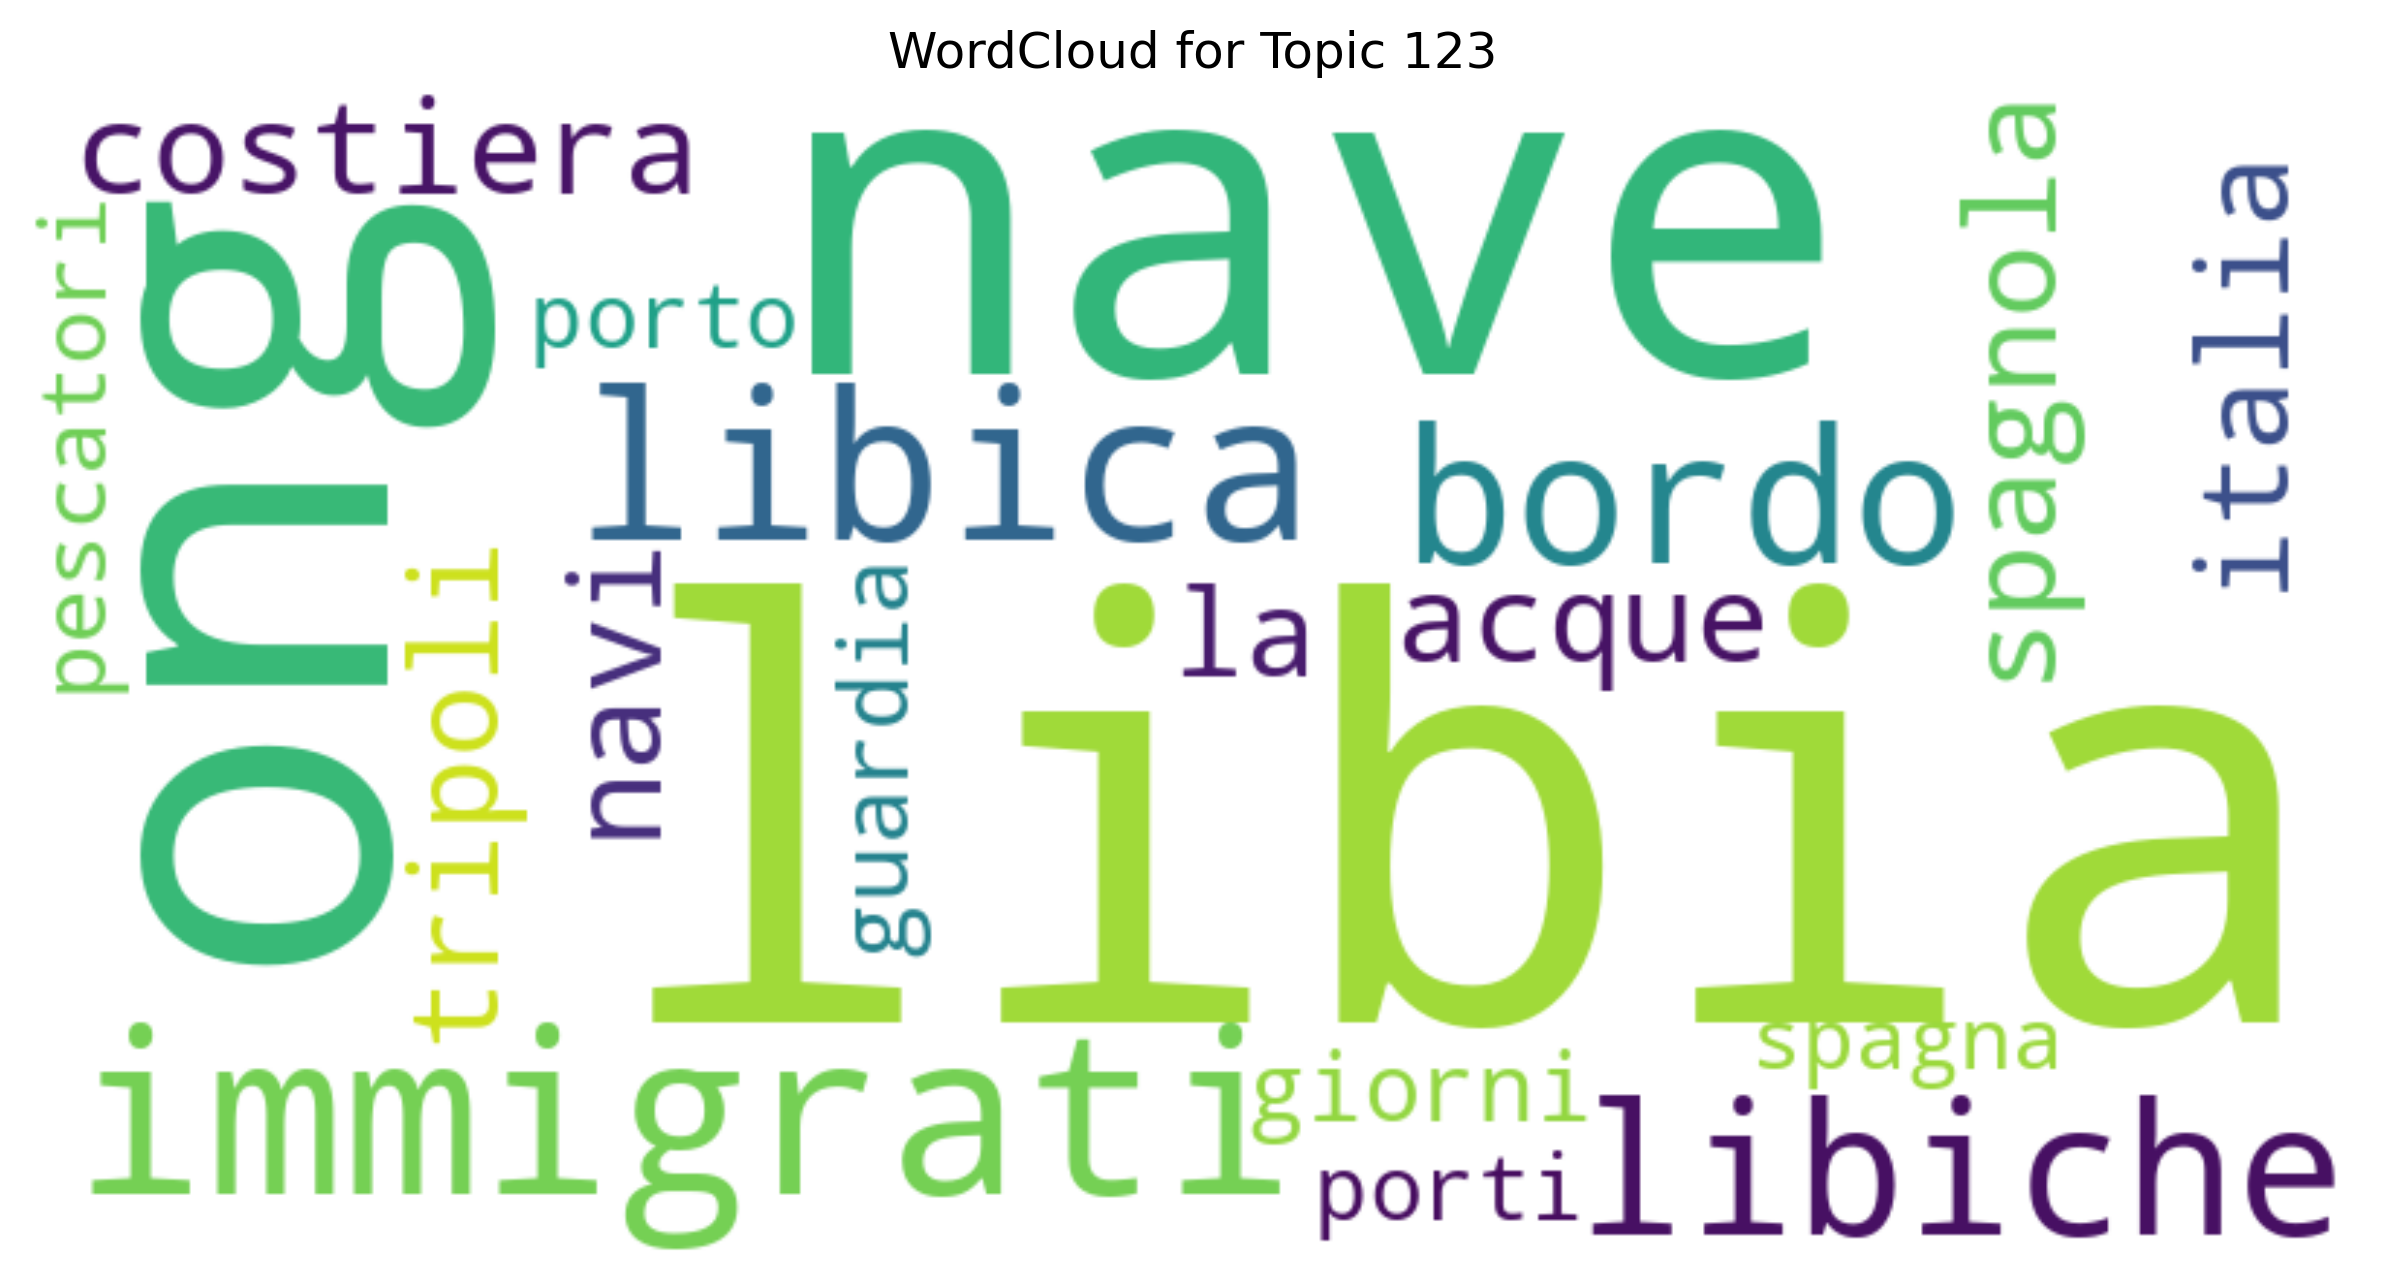
\includegraphics[width=1\linewidth]{wordcloud_topic_123.png}
    \caption{Word cloud representation of topic 123 (20th most frequent topic}
    \label{fig:topic123}
\end{figure}

\begin{figure*}[htbp]
    \centering
    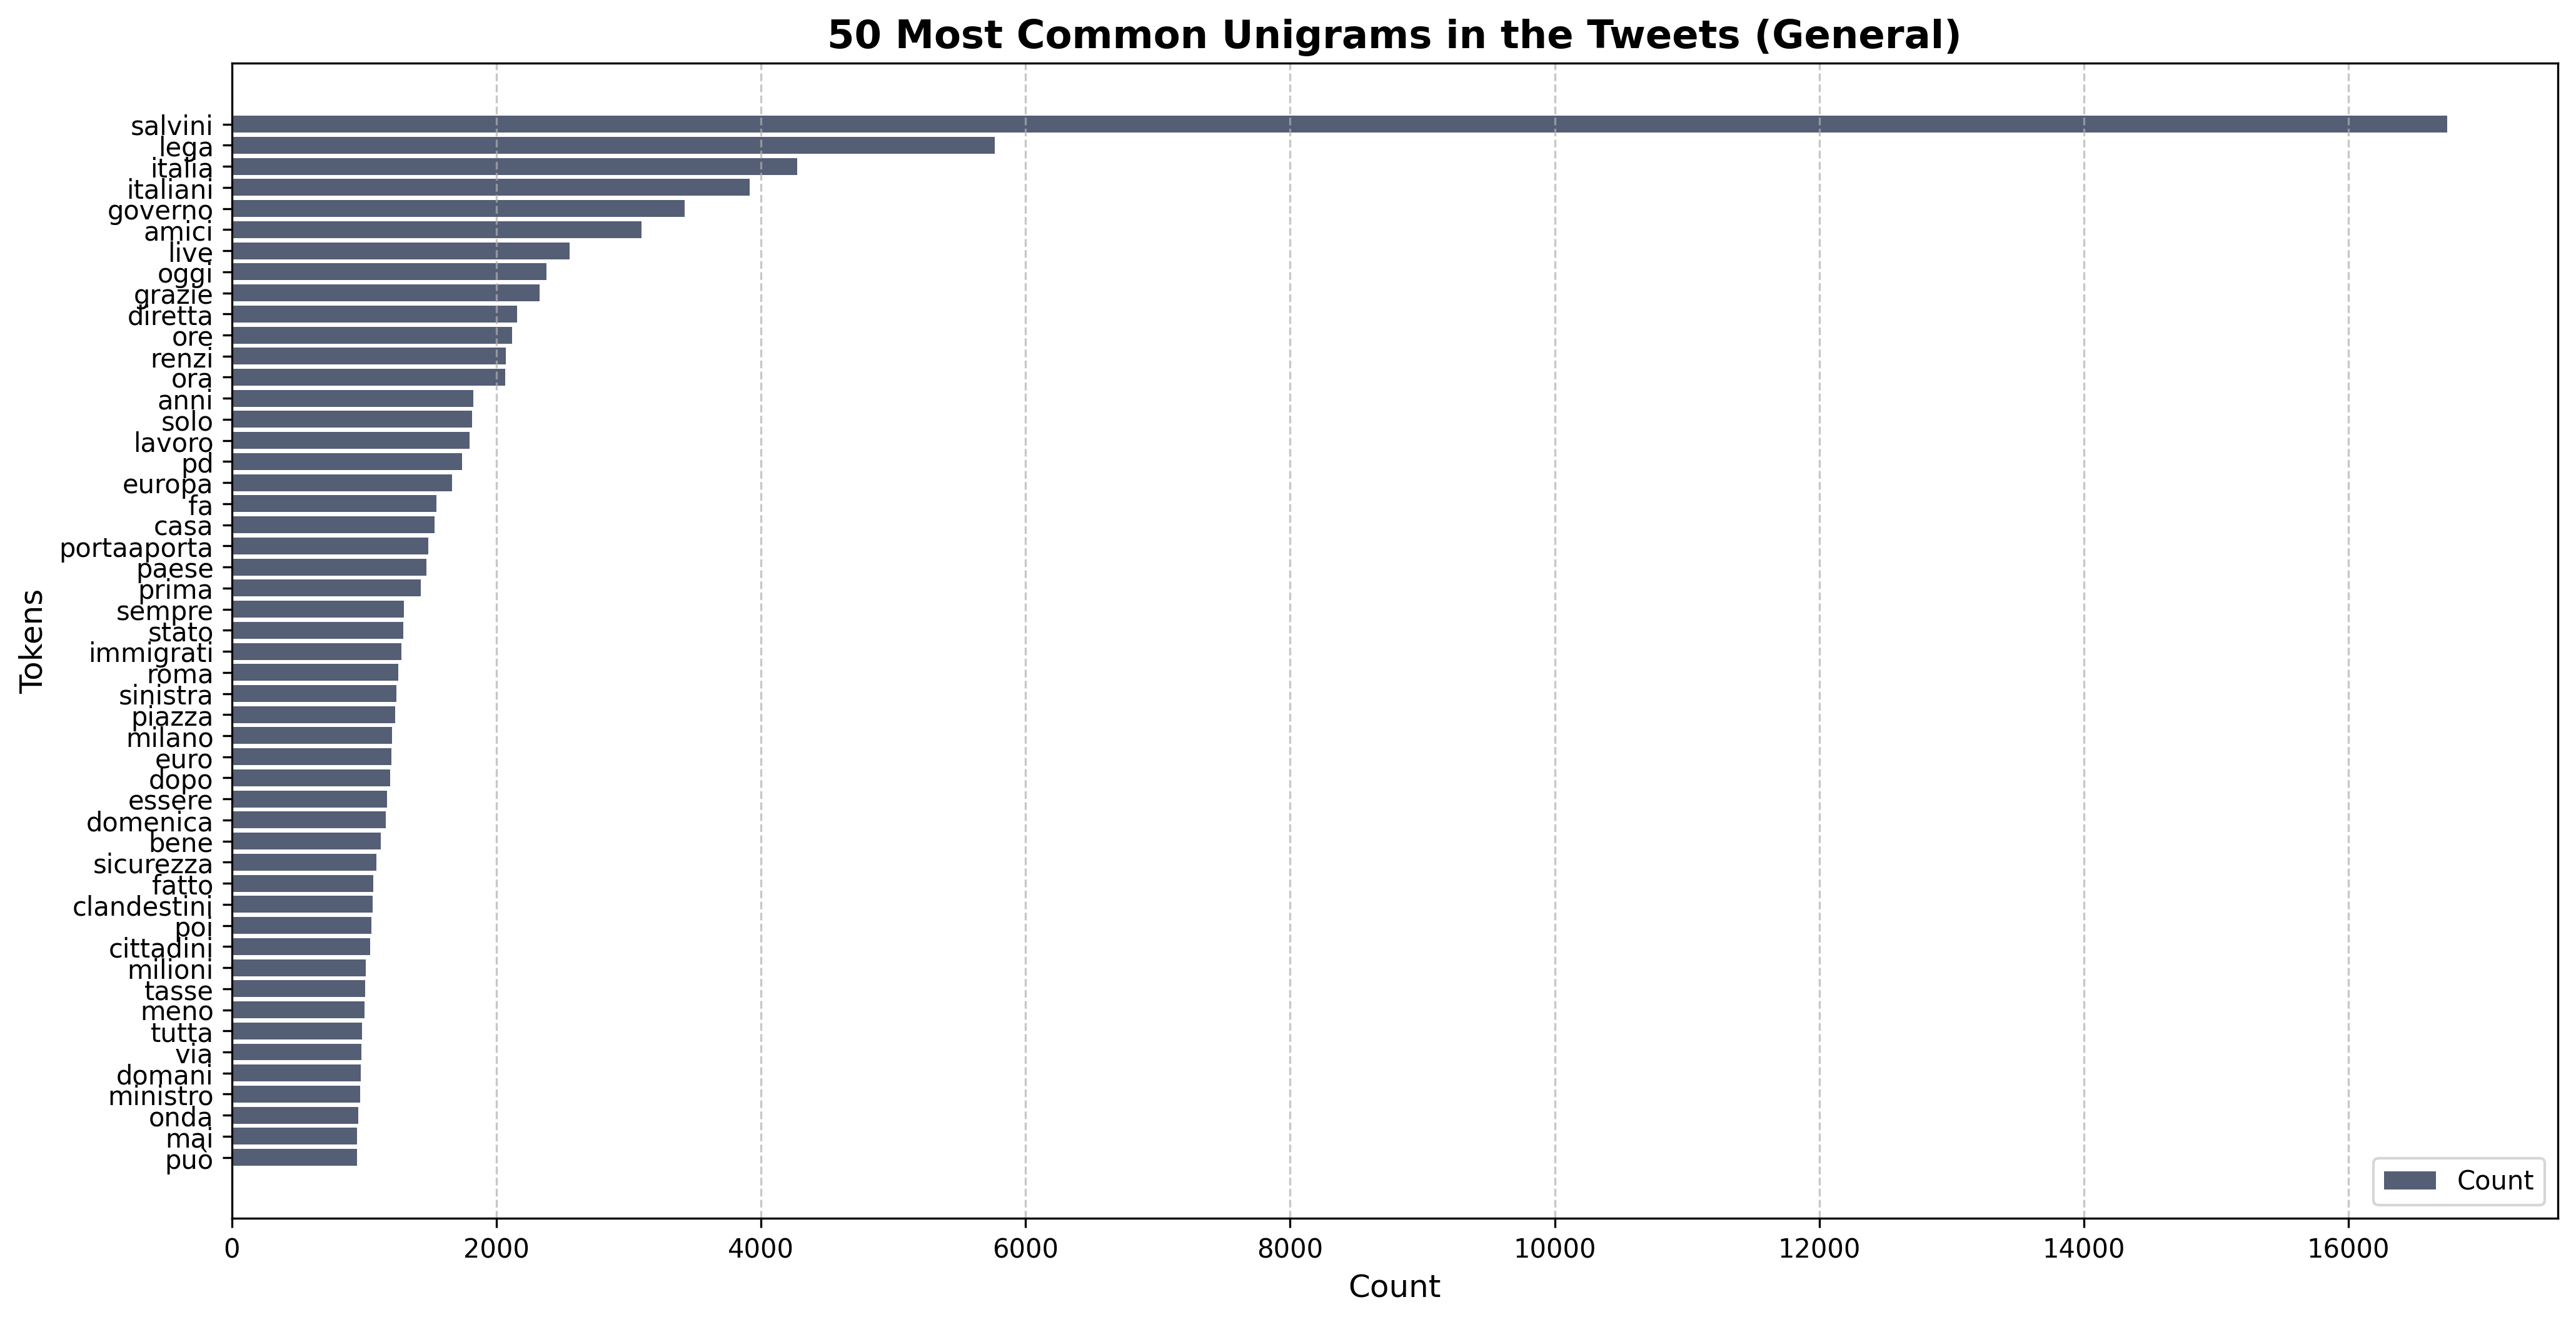
\includegraphics[width=1\linewidth]{50_most_common_unigrams_general.png}
    \caption{50 most common unigrams over the whole dataset}
    \label{fig:uni_gen}
\end{figure*}

\begin{figure*}[htbp]
    \centering
    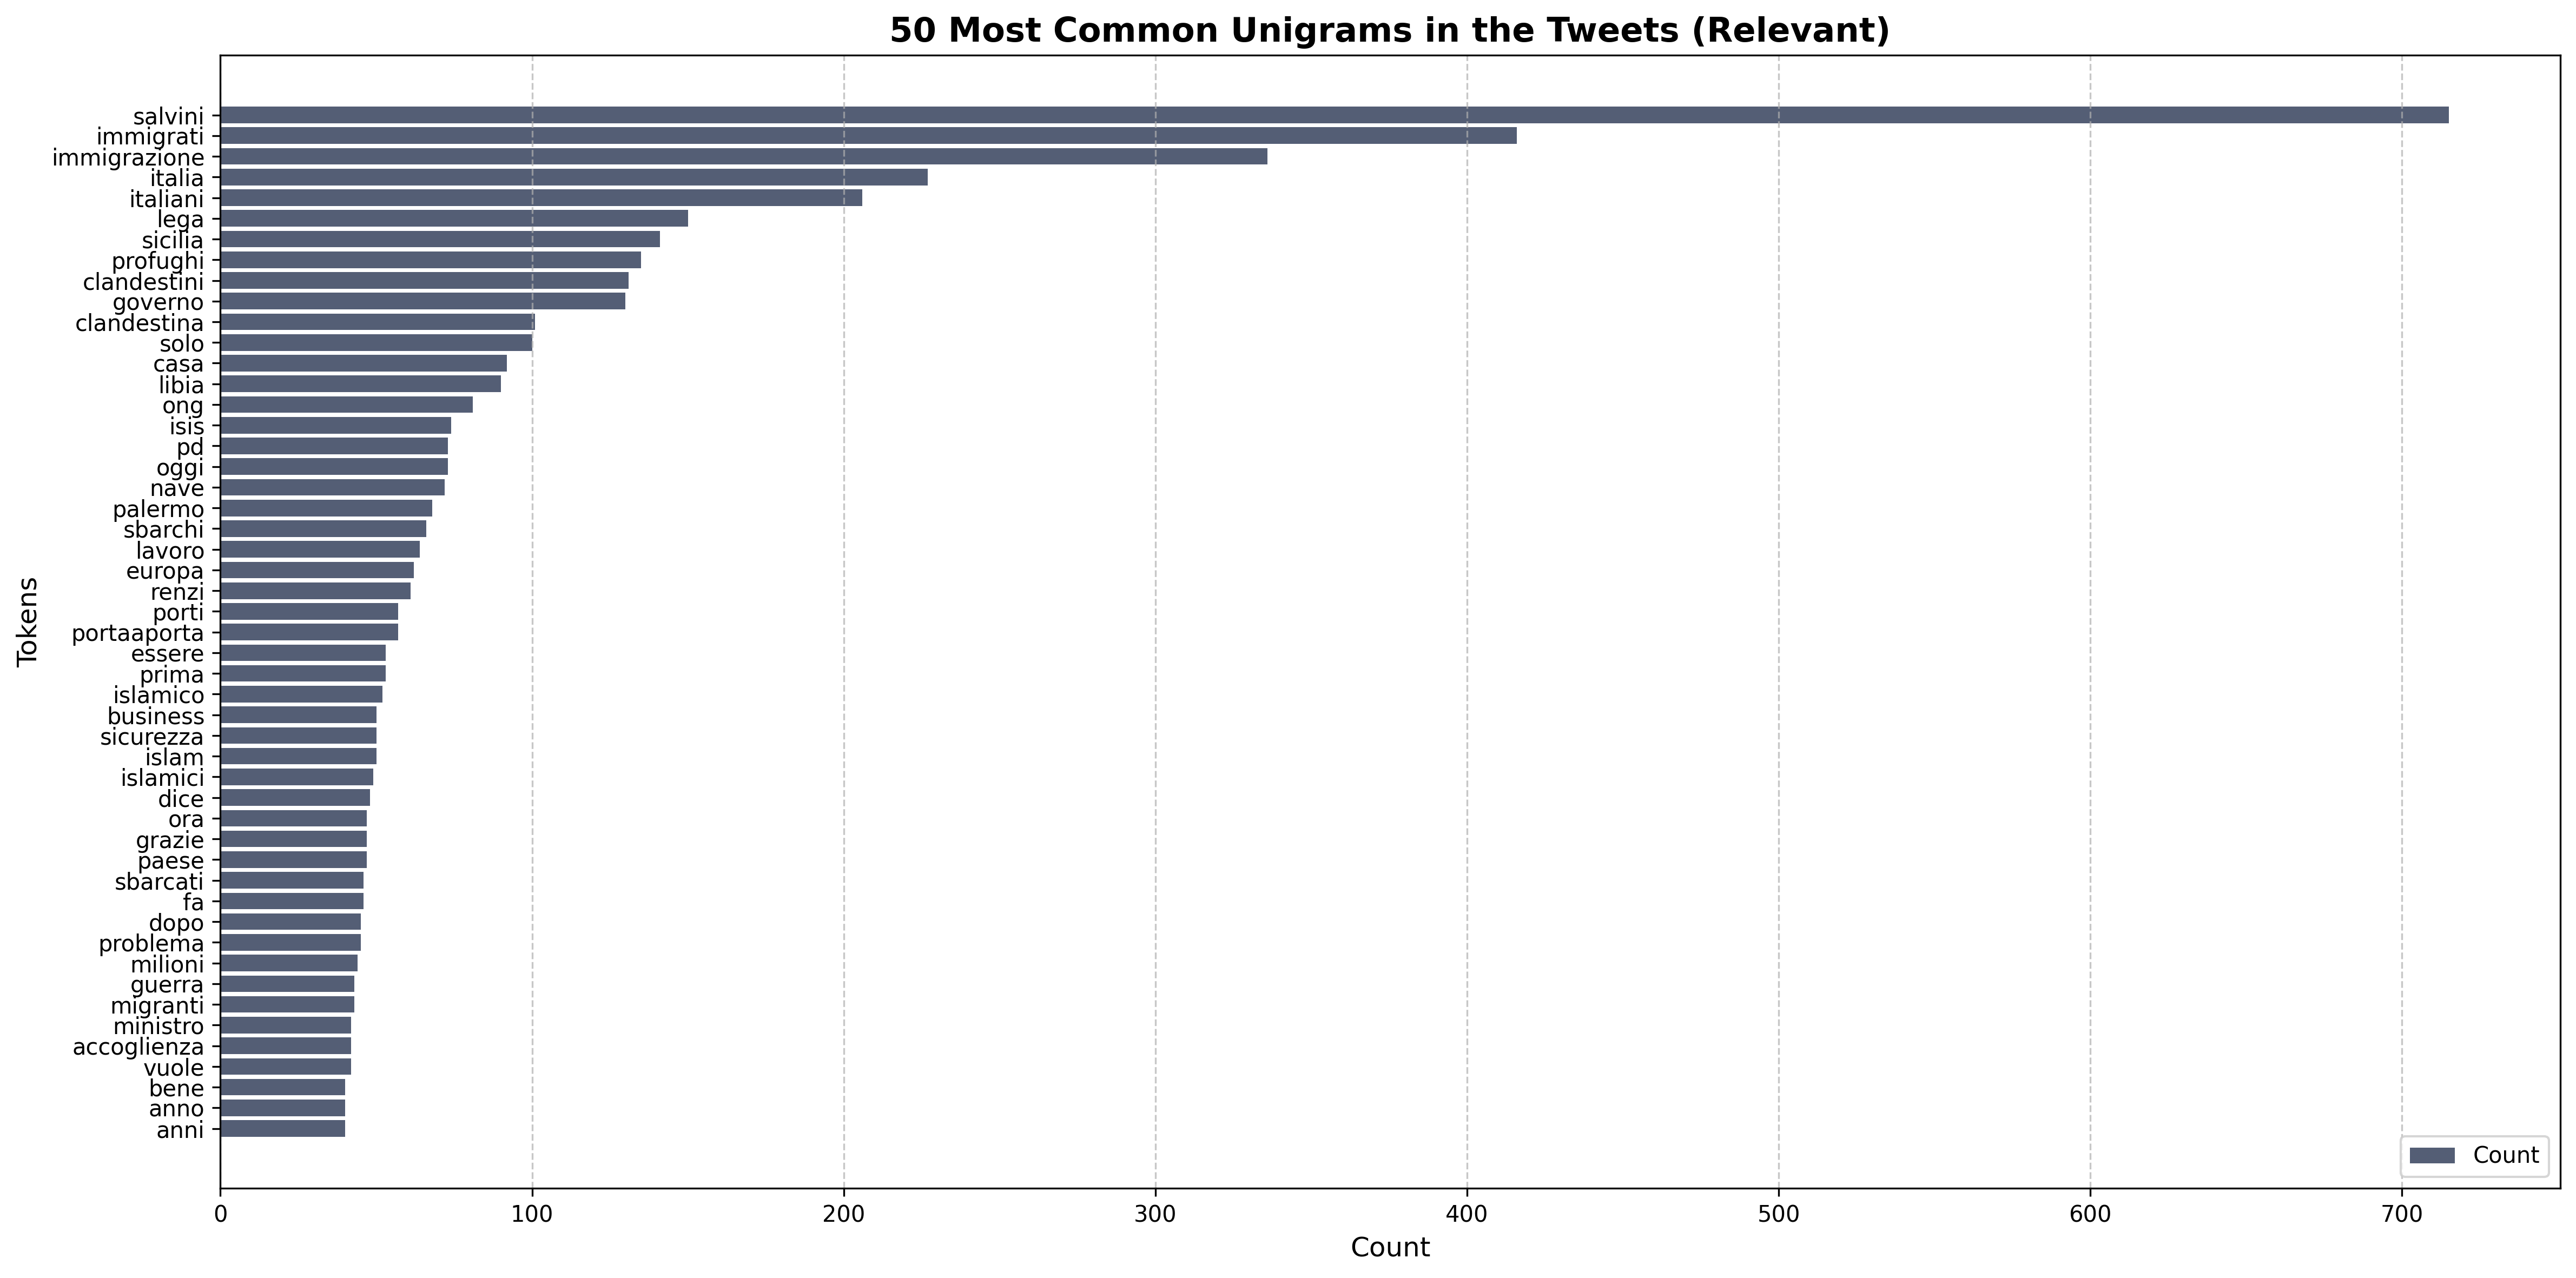
\includegraphics[width=1\linewidth]{50_most_common_unigrams_relevant.png}
    \caption{50 most common unigrams over the immigration-related tweets}
    \label{fig:uni_rel}
\end{figure*}

\begin{figure*}[htbp]
    \centering
    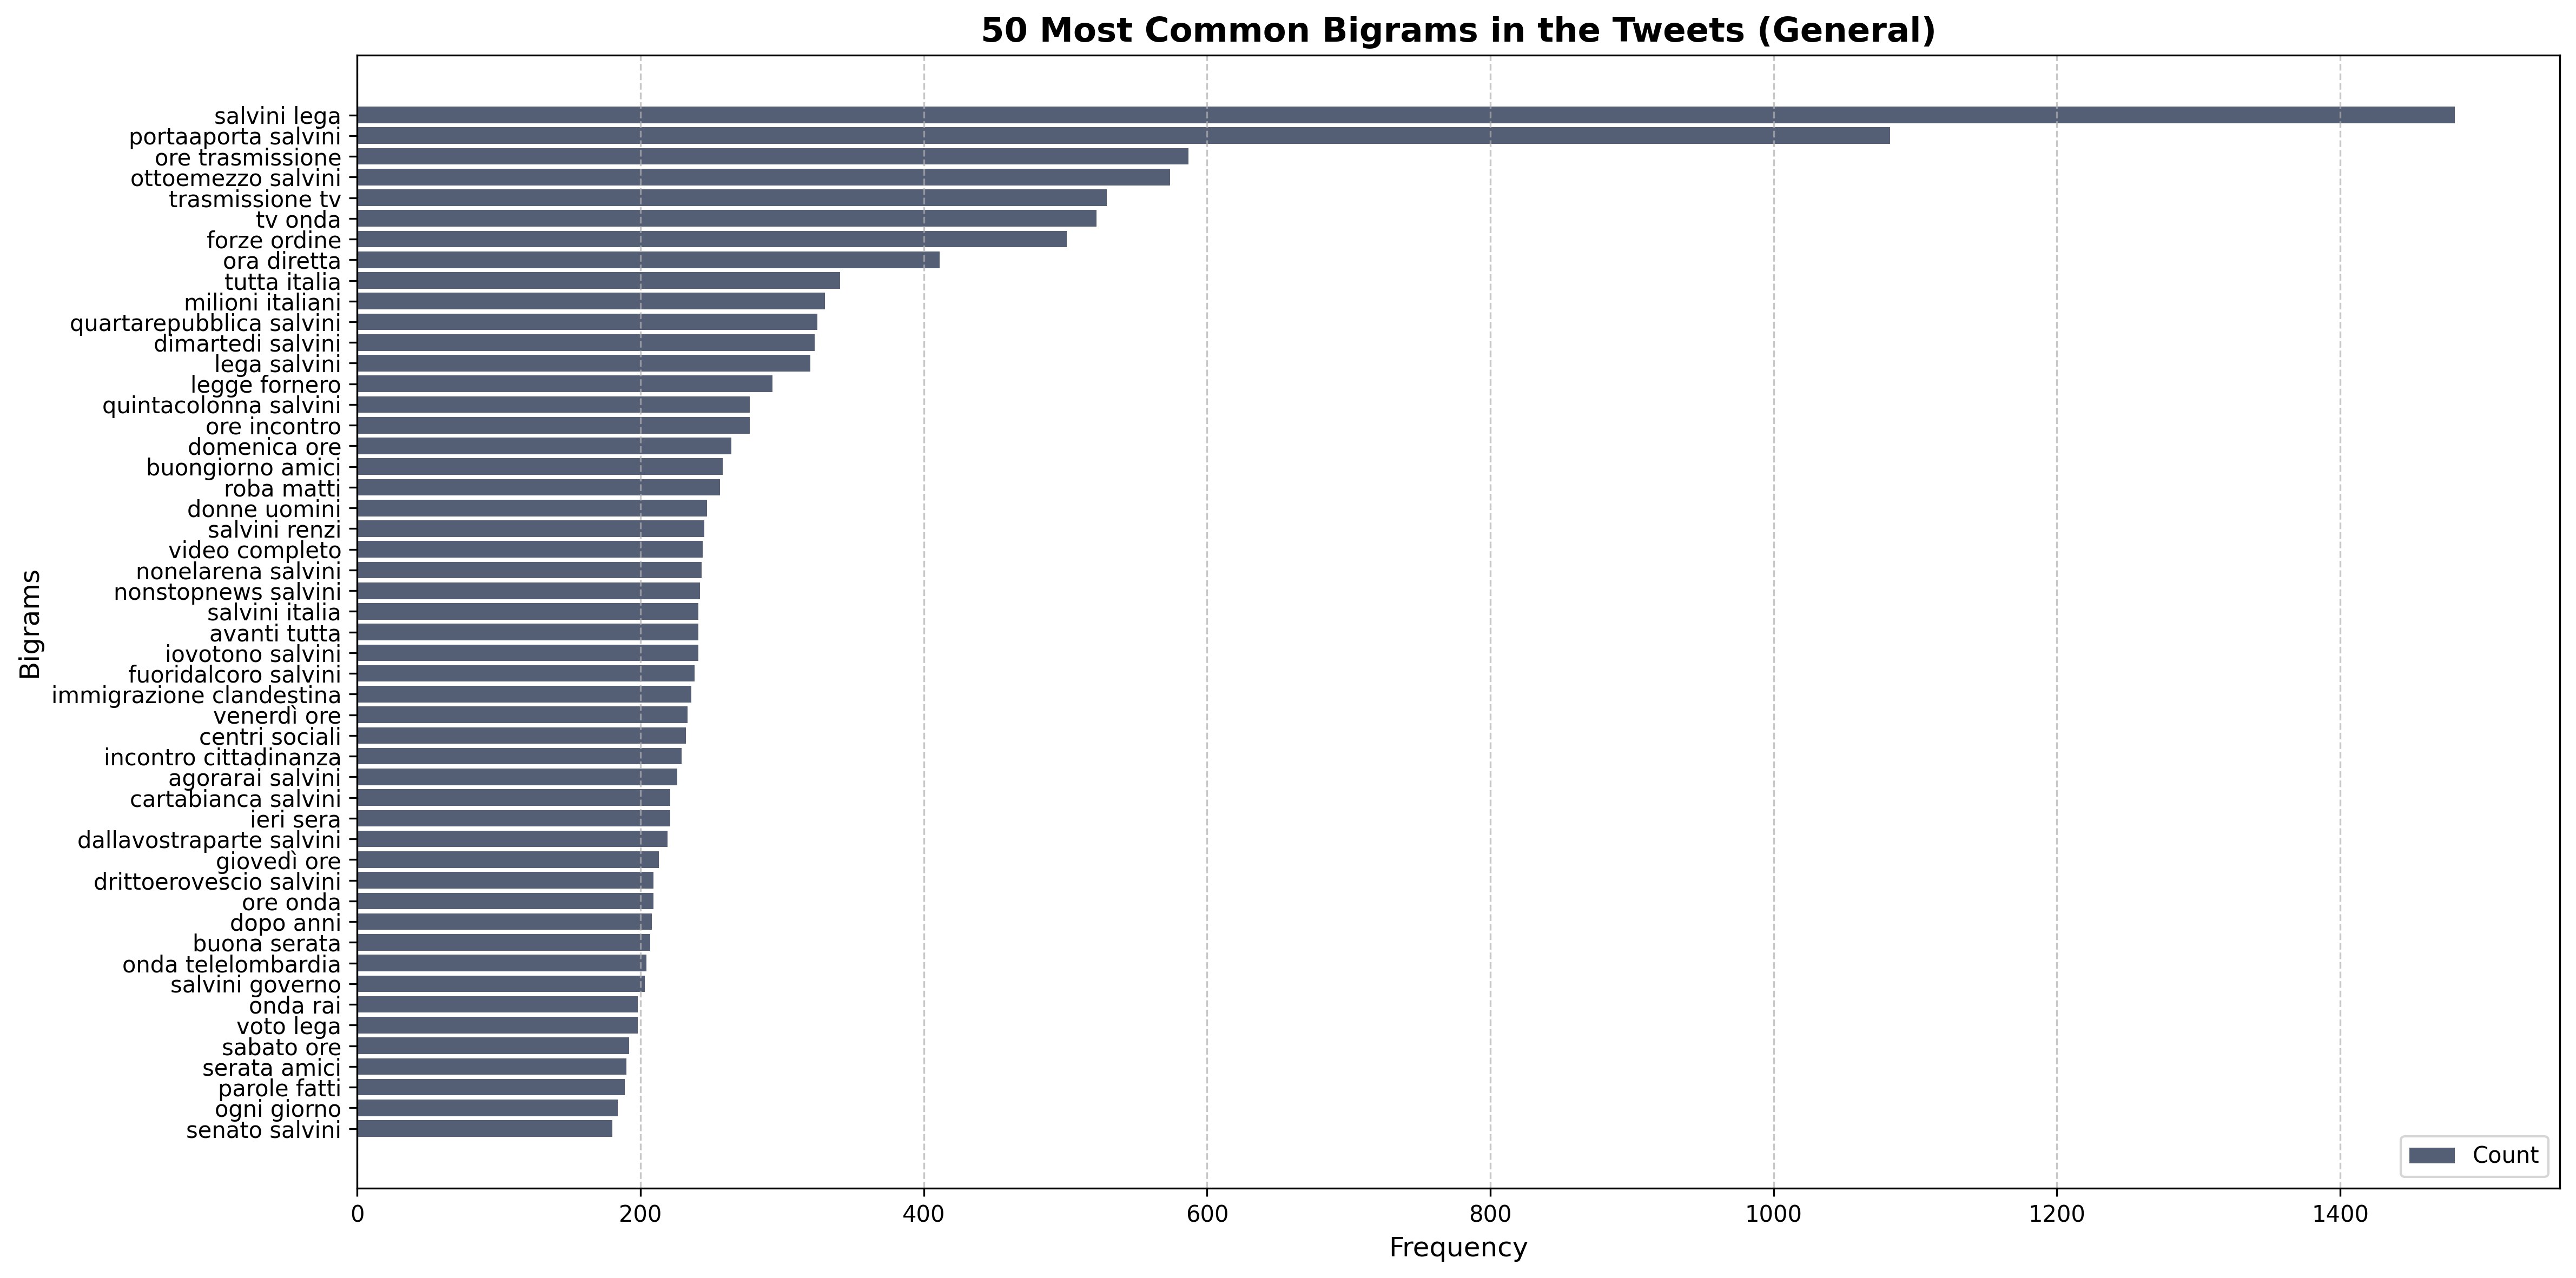
\includegraphics[width=1\linewidth]{50_most_common_bigrams_general.png}
    \caption{50 most common bigrams over the whole dataset}
    \label{fig:bi_gen}
\end{figure*}

\begin{figure*}[htbp]
    \centering
    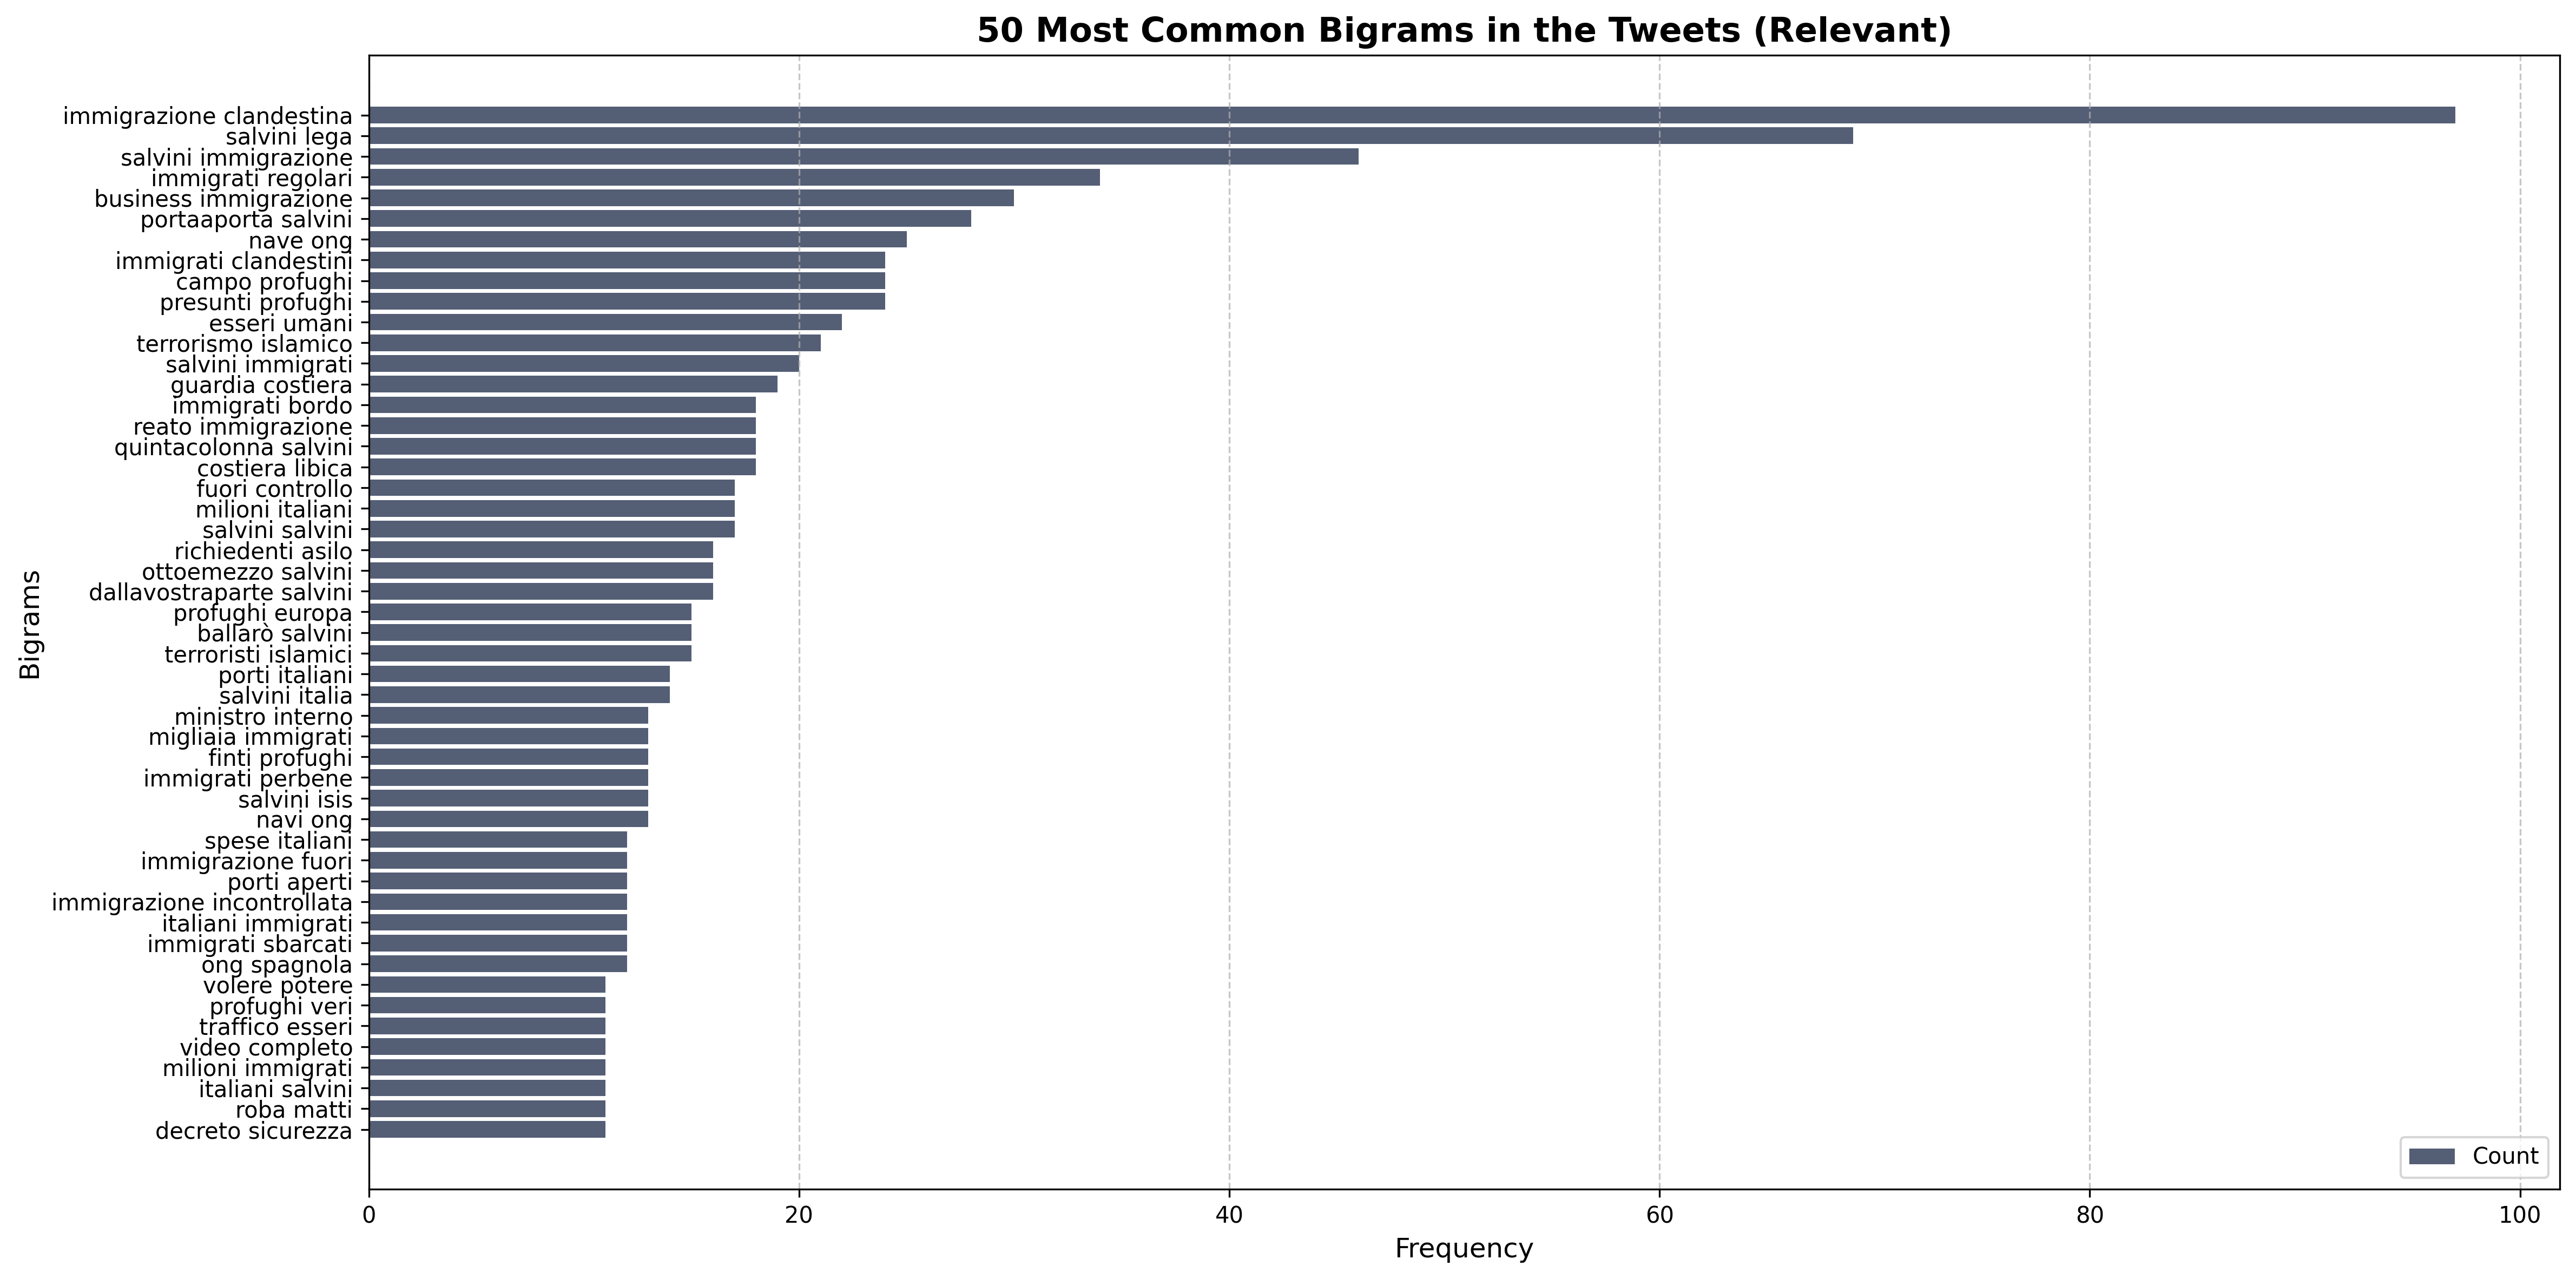
\includegraphics[width=1\linewidth]{50_most_common_bigrams_relevant.png}
    \caption{50 most common bigrams over the immigration-related tweets}
    \label{fig:bi_rel}
\end{figure*}

\begin{figure*}[htbp]
    \centering
    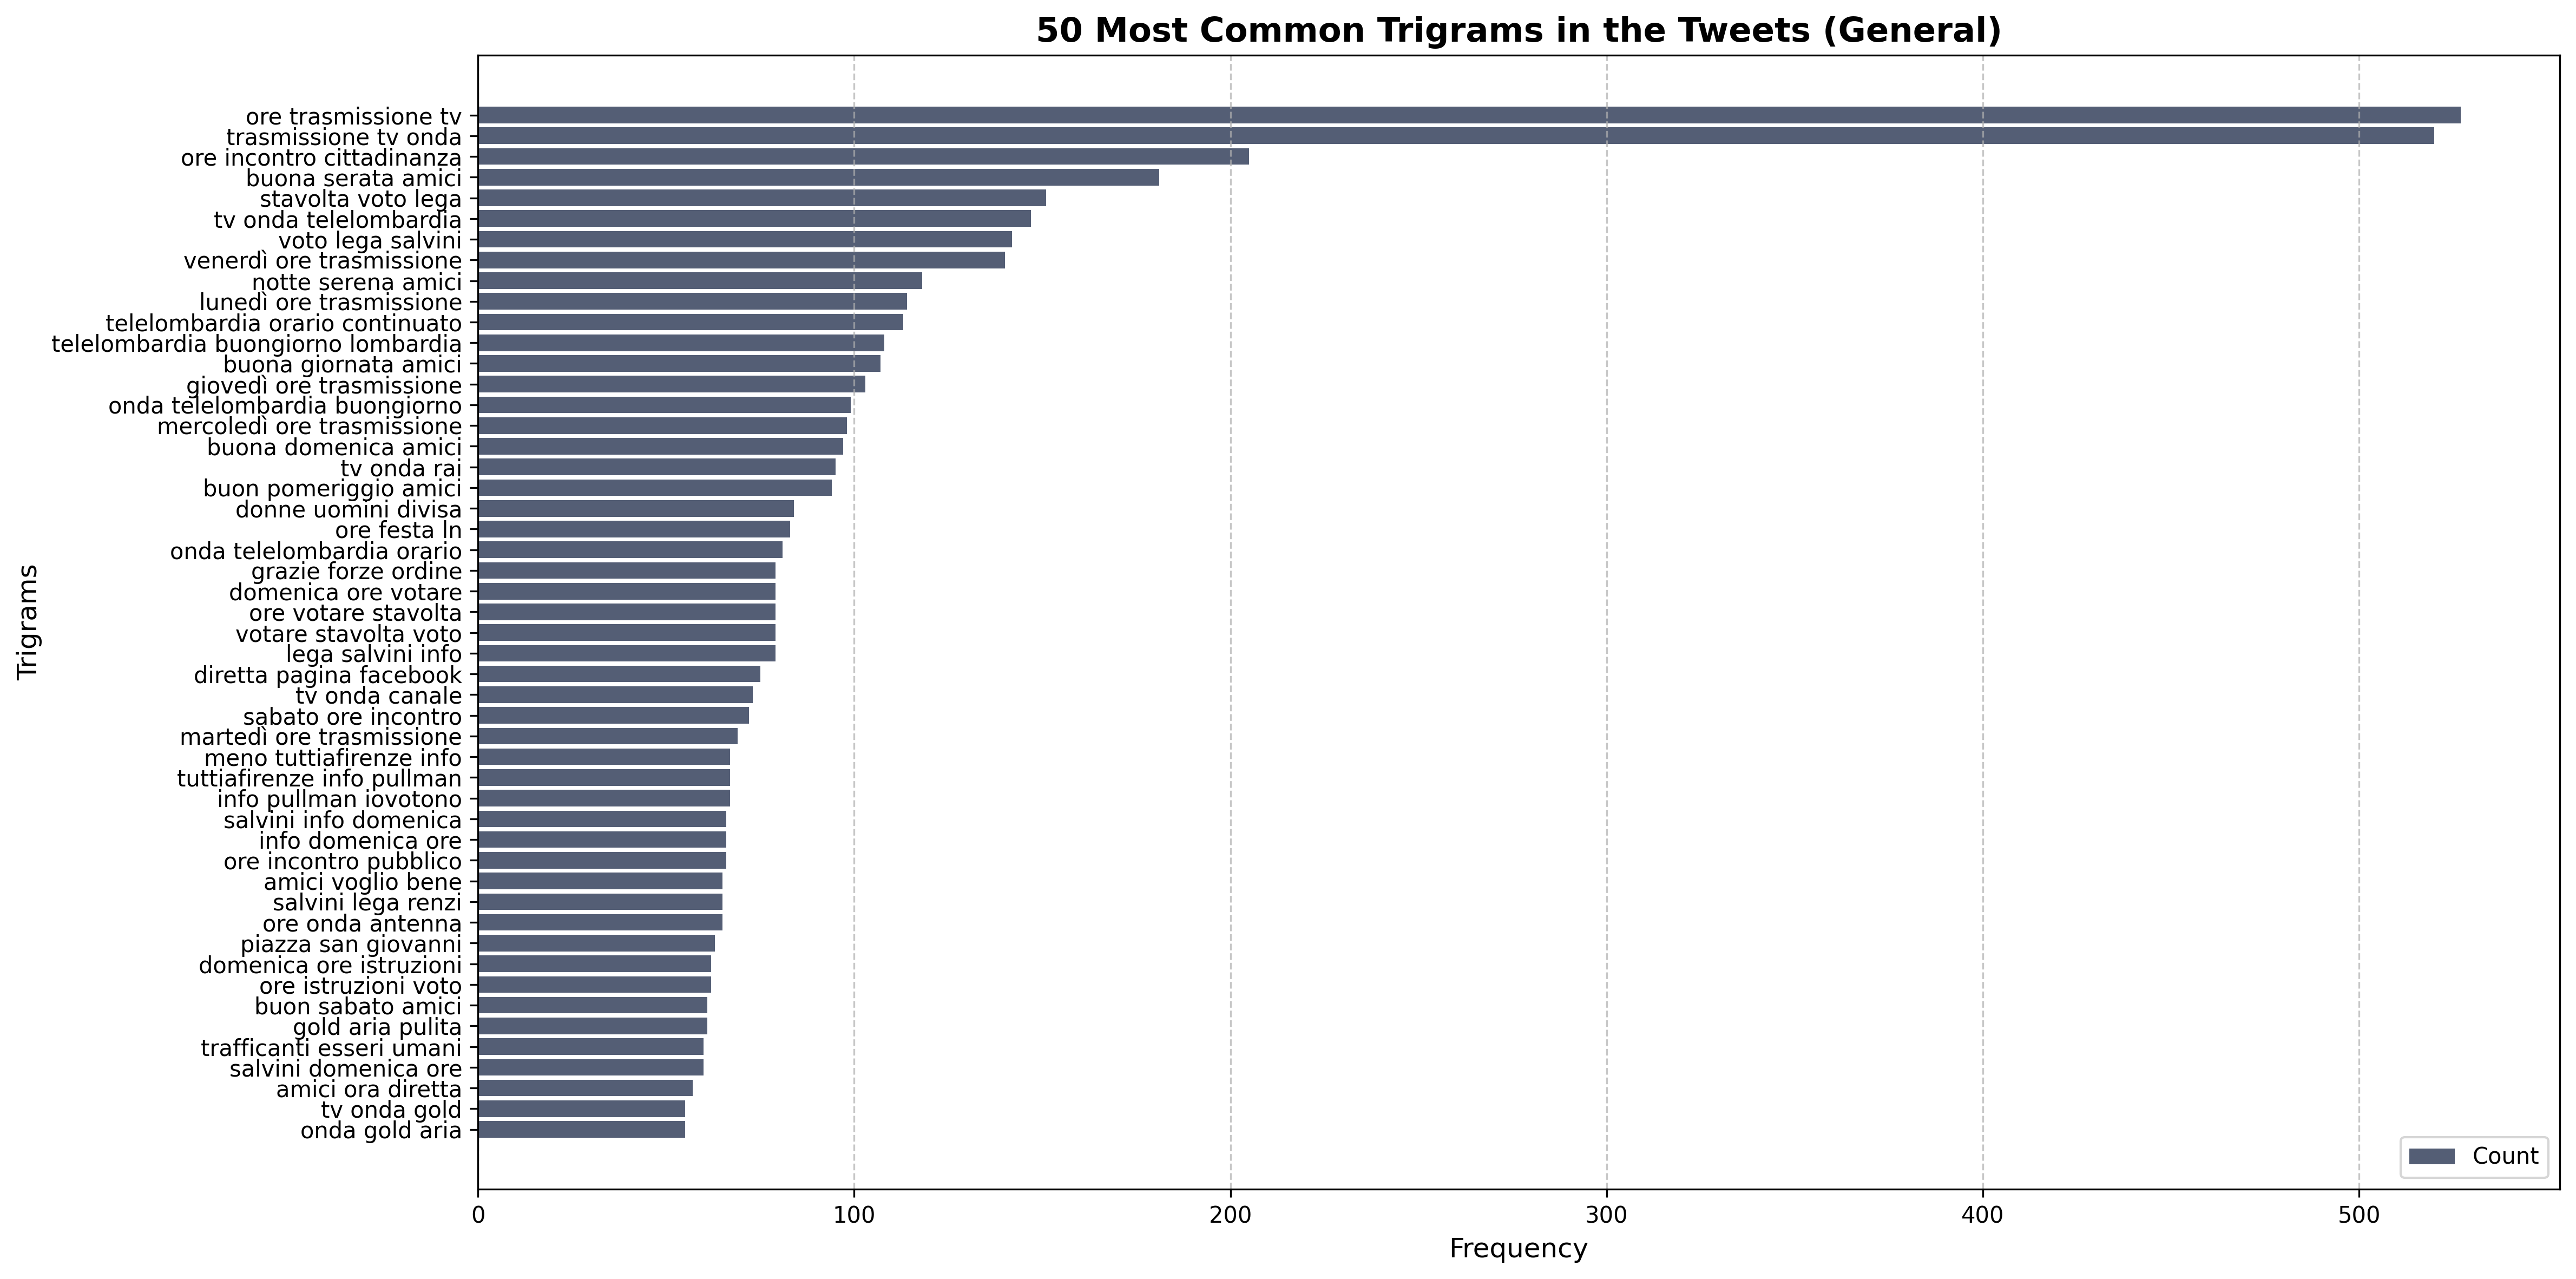
\includegraphics[width=1\linewidth]{50_most_common_trigrams_general.png}
    \caption{50 most common trigrams over the whole dataset}
    \label{fig:tri_gen}
\end{figure*}

\begin{figure*}[htbp]
    \centering
    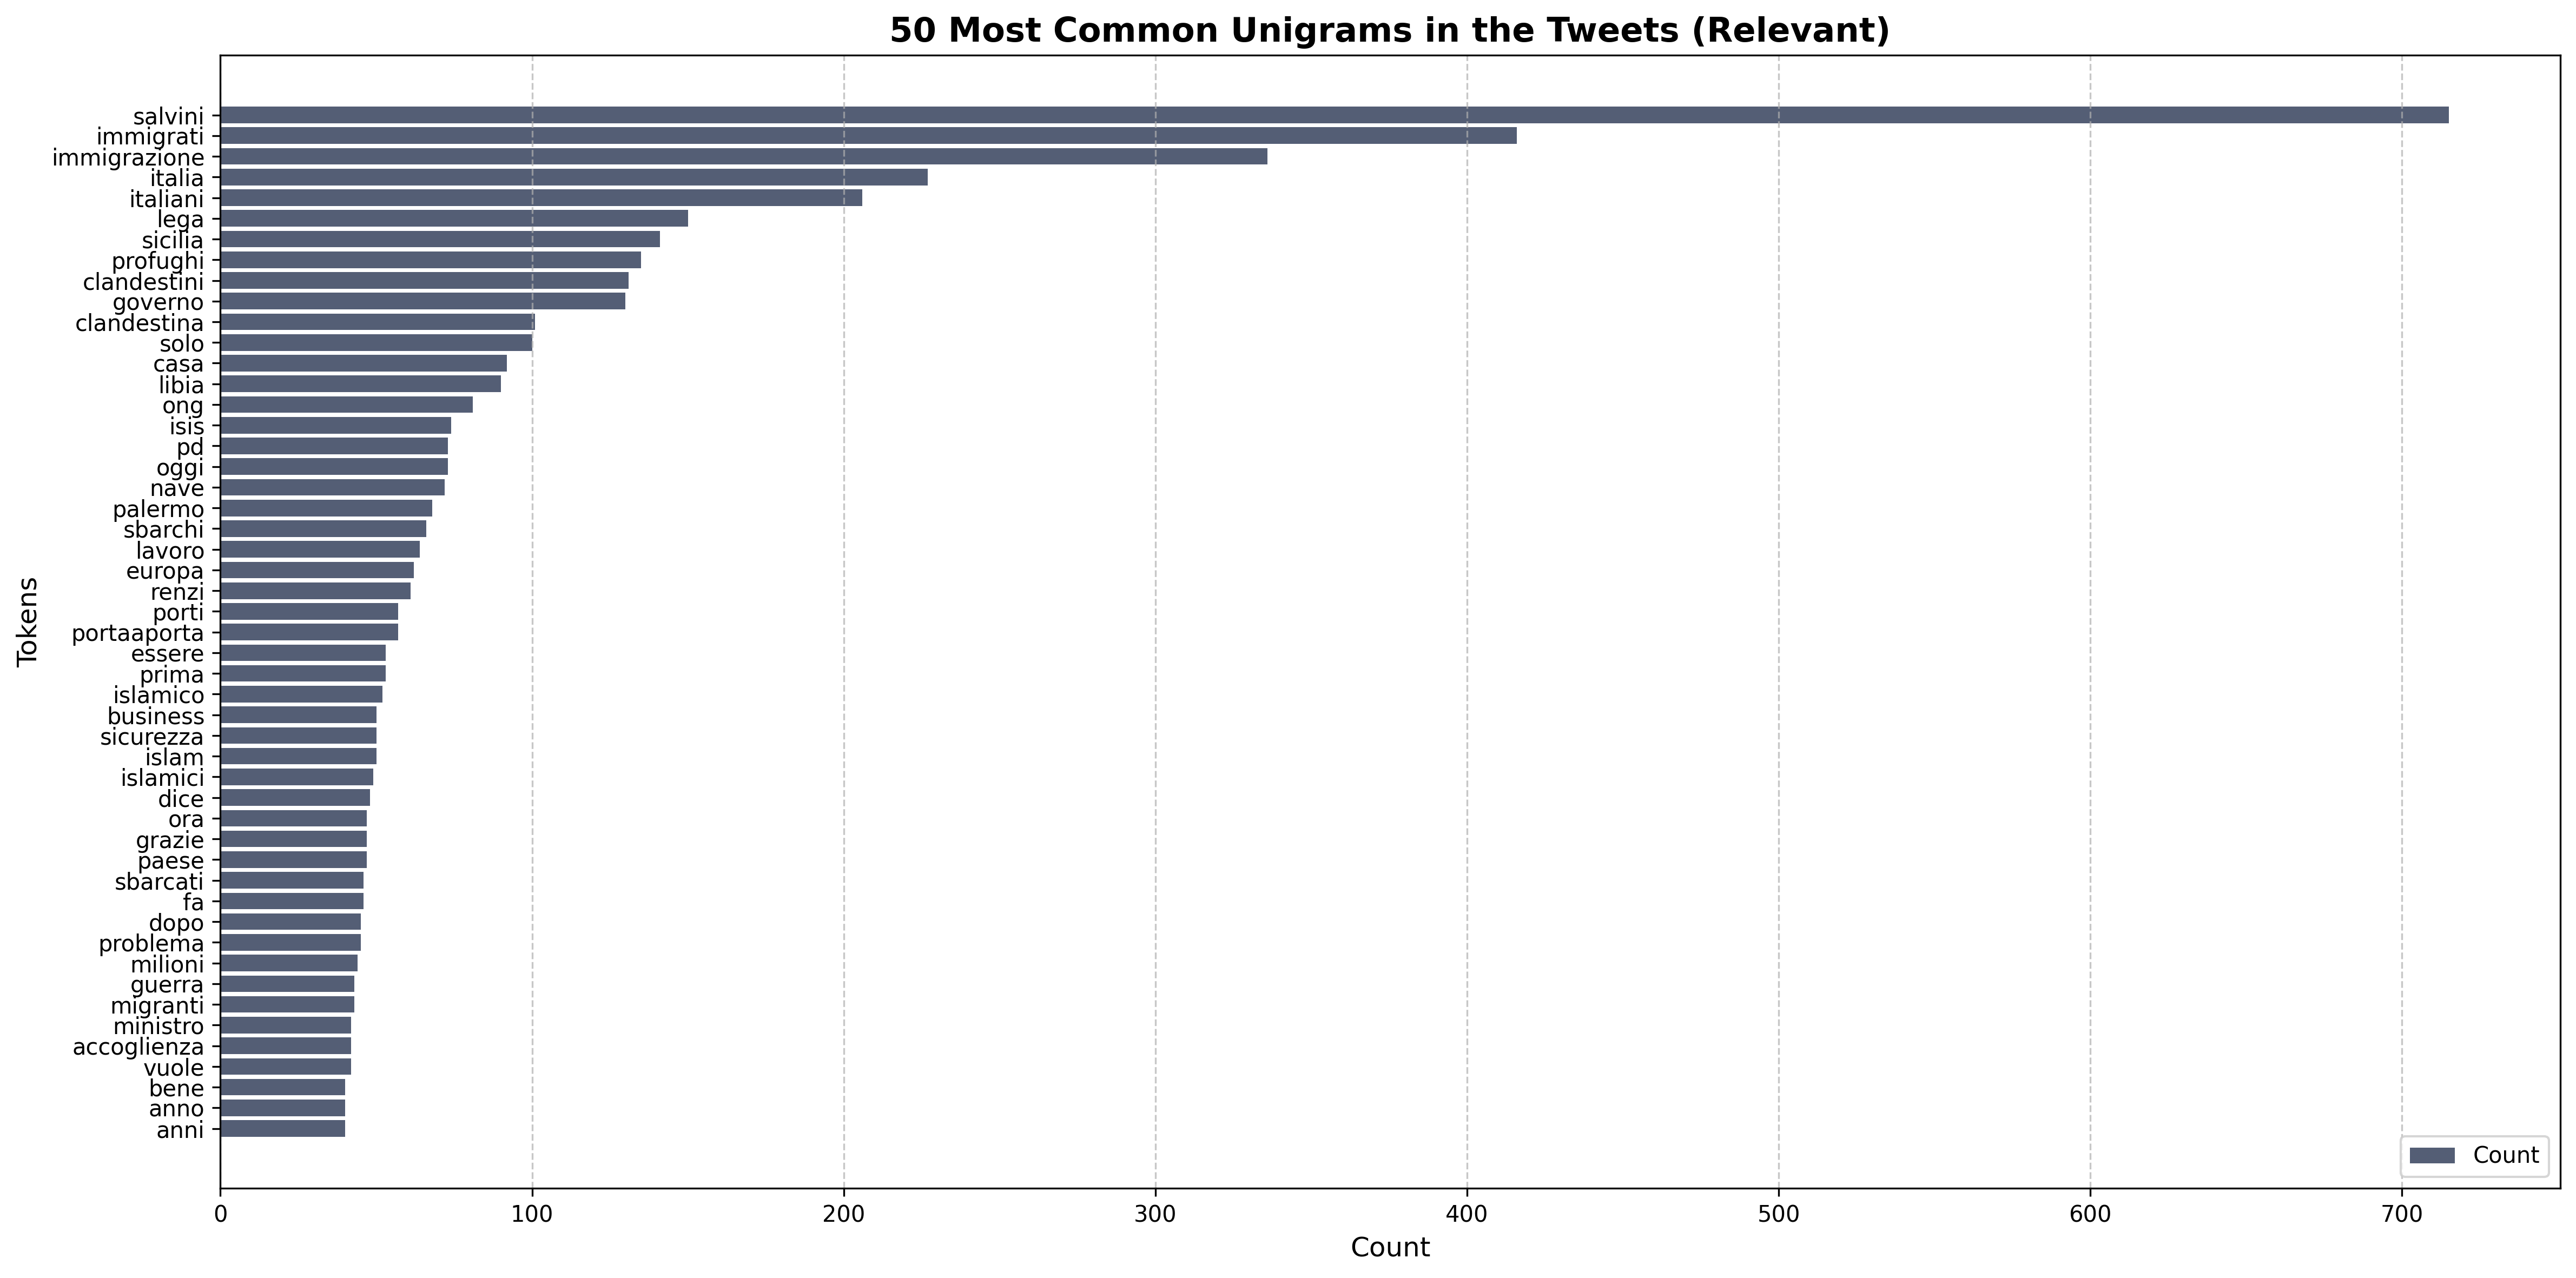
\includegraphics[width=1\linewidth]{50_most_common_unigrams_relevant.png}
    \caption{50 most common trigrams over the immigration-related tweets}
    \label{fig:tri_rel}
\end{figure*}


\begin{figure*}[htbp]
    \centering
    \includegraphics[width=1\linewidth]{Screenshot_20240714_164313.png}
    \label{fig:tri_rel}
\end{figure*}

\end{document}



